This chapter presents the simulation study results. We have seventy-two
simulation scenarios, as detailed in \autoref{cap:datasets}. For each
scenario we simulate 400 samples. In total, we fit 28800 models.

\section{SIMULATION STUDY}
\label{cap:simures}

Let us just recap the parameter values used
\begin{align*}
 \text{High CIF configuration}:~&\quad
 \{\beta_{1} = -2,~\beta_{2} = -1.5,~\gamma_{1} = 1,~\gamma_{2} = 1.5,~
   w_{1} = 3,~w_{2} = 4
 \};\\
 \text{Low CIF configuration}:~&\quad
 \{\beta_{1} = 3,~\beta_{2} = 2.5,~\gamma_{1} = 2.6,~\gamma_{2} = 4,~
   w_{1} = 5,~w_{2} = 10
 \}.
\end{align*}
\begin{minipage}{0.15\textwidth}
 \begin{align*}
  \sigma_{u_{1}}^{2}   &= 1\\
  \sigma_{u_{2}}^{2}   &= 0.7,\\
  \sigma_{\eta_{1}}^{2} &= 0.6\\
  \sigma_{\eta_{2}}^{2} &= 0.9
 \end{align*}
\end{minipage}%
\begin{minipage}{0.85\textwidth}
 \[
  \text{Correlation structure}~=~\begin{blockarray}{ccccc}
                                  u_{1} & u_{2} & \eta_{1} & \eta_{2}\\
                                  \begin{block}{(cccc)c}
                                   1 & 0.1 & -0.5 &  0.3 & u_{1}\\
                                     &   1 &  0.3 & -0.4 & u_{2}\\
                                     &     &    1 &  0.2 & \eta_{1}\\
                                     &     &      &    1 & \eta_{2}\\
                                  \end{block}
                                 \end{blockarray}.
 \]
\end{minipage}

\vspace{0.3cm}
\noindent
The parameter values per se are not important. What is important is to
keep in mind the behaviors implied by them, and see if the proposed
model is able to learn the true values in several different scenarios
and measure the quality of this learning.

The take-home message for the fixed-effect parameters, is to show that
we can construct different level CIF scenarios. The \(\bm{\beta}\)s are
responsible for the curve maximum point or plateau, the \(\bm{\gamma}\)s
and \(\bm{w}\)s are responsible for basically the curve shape. Its
interpretation is presented in detail in \autoref{cap:model}. About the
latent-effects, the chosen covariance structure is considerably high but
still acceptable. The underlying idea was to try to build a realistic
covariance scenario and consequently be able to check how the model
performs in such conditions.

In the following pages we have several graphs summarizing the parameters
bias. In each figure, we have the parameter bias and its uncertainty
described by a Wald-based interval i.e., \(\pm\) 1.96 the bias standard
deviation. This is a good uncertainty representation choice since it is
symmetric and robust to outliers. In the \autoref{cap:appendixD}, we
have the same parameters bias but with the corresponding 2.5 and 97.5\%
quantiles. We chose to use these uncertainty representations uniquely
based on the point estimates instead of the standard error
computations. In several scenarios, the model fails to compute all the
standard errors, caused by Hessian instability problems.

The seventy-two scenarios are accommodated. We have up to four blocks of
bars, each block representing a model. In each block we have eighteen
bars, each bar representing the 400 fits in each of the eighteen
scenarios, \(4 \times 18 \times 400 = 28800\). 

Each scenario name consists of a combination of three strings
\begin{itemize}
 \item The cluster size (cs), 2, 5, and 10;
 \item The CIF configuration, high and low;
 \item The sample size, 5, 30, and 60 thousand.
\end{itemize}
We have tried to fit a total of 28800 models but not all
converged. Besides that inconvenience, from the ones that converged do
not all converged in the strict sense of the word. To show these two
characteristics respectively, we control the bar widths and colors. The
ideal convergence is the traditional one i.e., based on the
gradient. However, in complicated optimization scenarios as the one we
are here, we can reach a convergence based on a metric different from
the gradient one.

In the \texttt{base::nlmimb()} \texttt{R}'s \texttt{PORT}
implementation, when the default gradient-based convergence is reached
we get a 0 flag message. When the optimization converges but not
gradient-based, we get a 1 flag message. Looking at the technical report
of \citeonline{PORTreport}, we see that this different convergence means
that the last algorithm iterate \(x\) appears to be at a certain scaled
distance of the locally optimal point \(x^{\ast}\). This scaled
distance, \(p(x, x^{\ast})\), is defined by
\[
 p(x, y) =
 \underset{1~\leq i~\leq~p}{\text{max}}
 \left\{d_{i}, |x_{i} - y_{i}|\right\}
 \Big/
 \underset{1~\leq j~\leq~p}{\text{max}}
 \left\{d_{j}, |x_{j}| + |y_{j}|\right\},
\]
where \(d\) is a certain scale vector. In all figures, the presented
convergence percentage is from the gradient-based one.

Something specific can be said about each parameter but let us keep the
focus on the general remarks. Starting from the fixed-effect parameters
in \autoref{fig:biassdbeta1}, \autoref{fig:biassdbeta2},
\autoref{fig:biassdgama1}, \autoref{fig:biassdgama2},
\autoref{fig:biassdw1}, and \autoref{fig:biassdw2}, we have very nice
results that already show a strong inclination towards the complete
model's choice.

With a latent structure only in the risk level or in the trajectory time
level, the low CIF scenarios are the ones with a much smaller
bias-variance. In general, the mean-bias is small but the variances are
high. When we have a latent structure on both levels but we still assume
the cross-correlations as zero (block-diag model), the results get a
little bit better. Nevertheless, when we assume a non-zero
cross-correlation structure (complete model), basically everything
changes for the better. The mean biases get even closer to zero, the
standard deviations decrease 50\% or more, and mainly, now the high CIF
scenarios are the ones with a much smaller bias-variance. All this is
accomplished through the consideration of the cross-correlations.

\begin{figure}[H]
 \setlength{\abovecaptionskip}{.0001pt}
 \caption{PARAMETER \(\beta_{1}\) BIAS WITH \(\pm\) 1.96 STANDARD
          DEVIATIONS}
 \vspace{0.2cm}\centering
 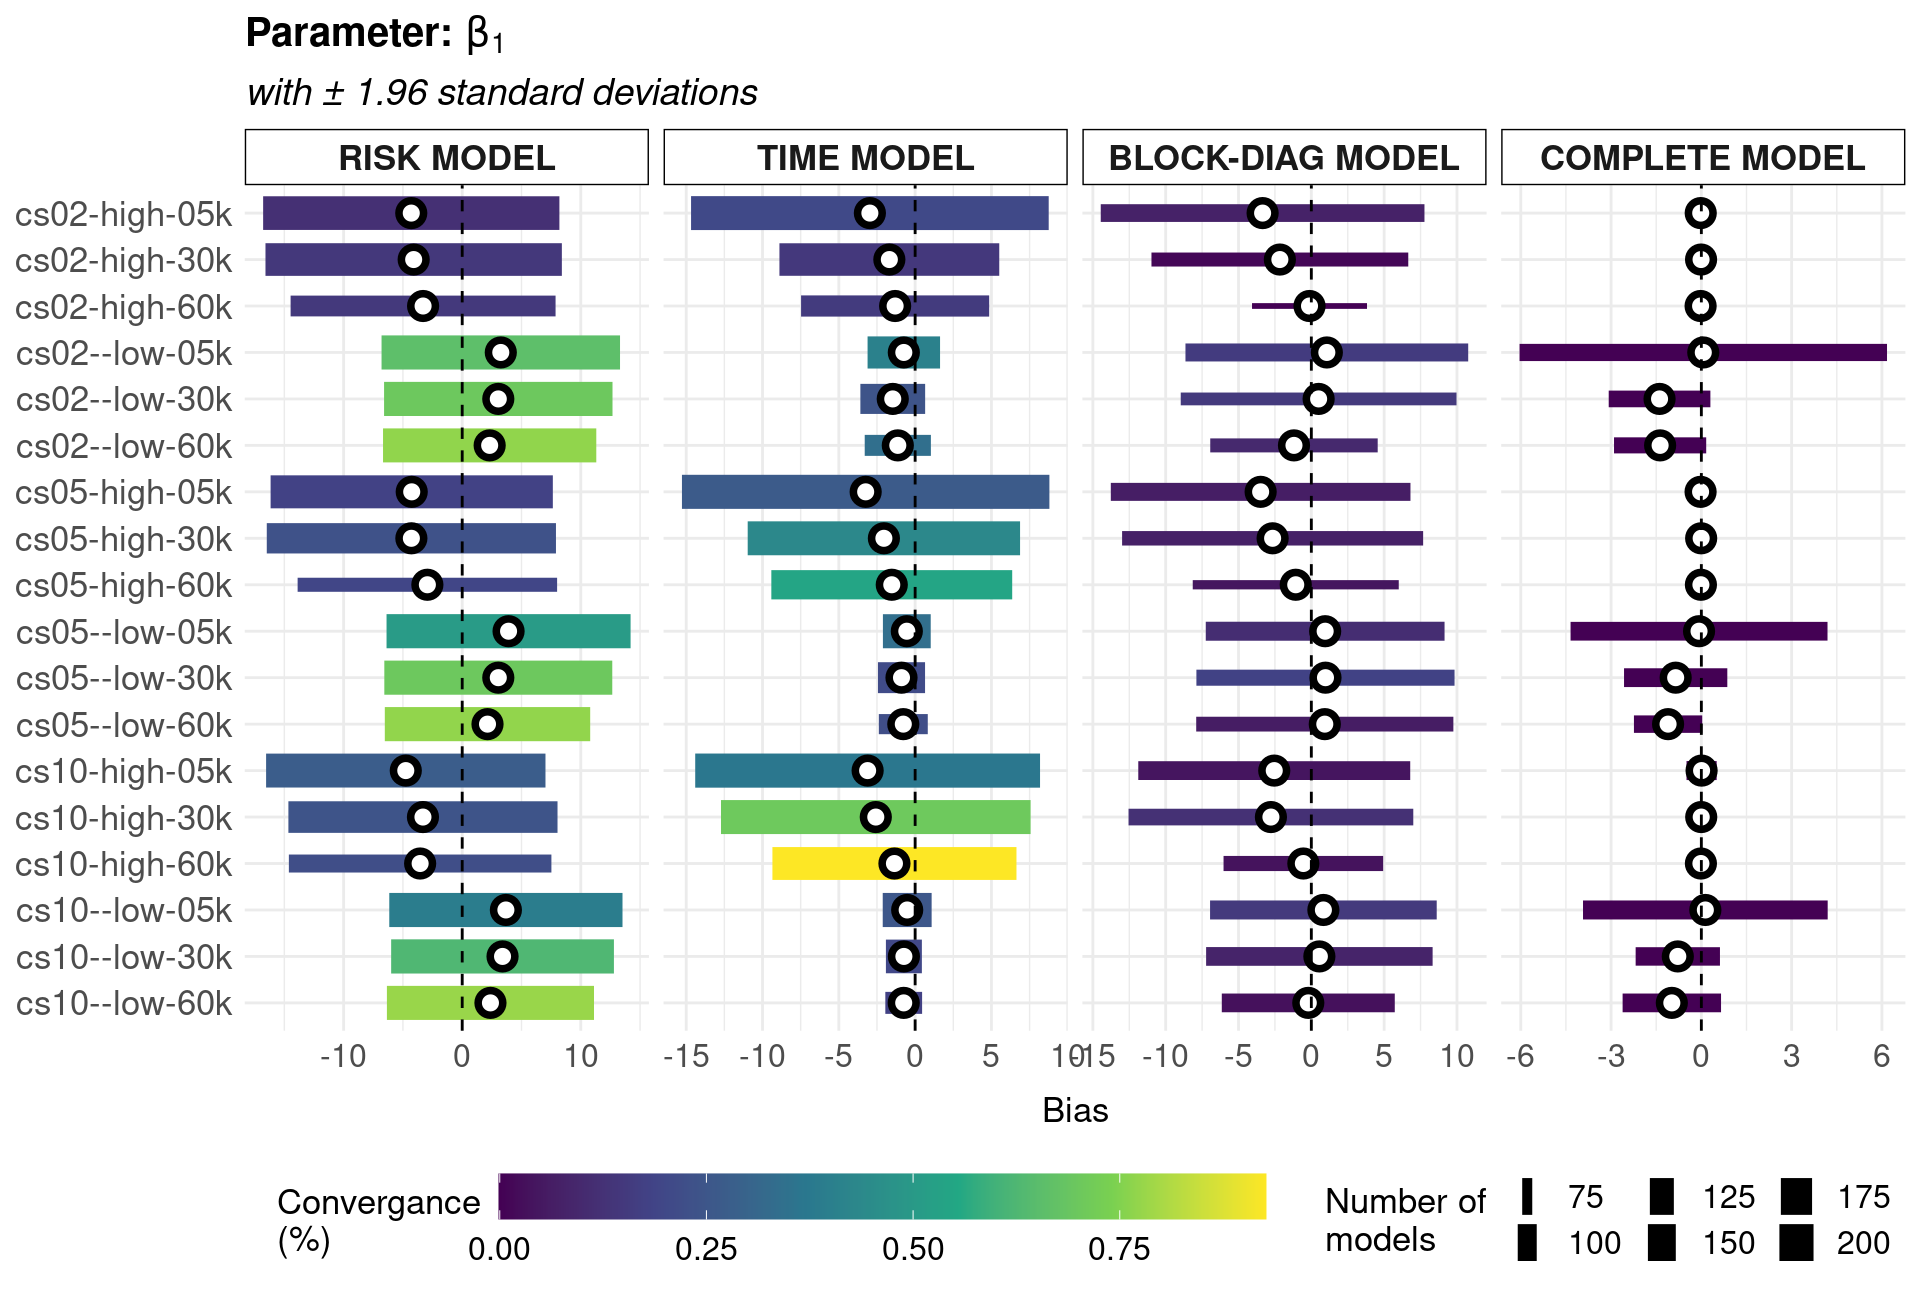
\includegraphics[width=\textwidth]{bias2plotsd-1.png}\\
 \begin{footnotesize}
  SOURCE: The author (2021).
 \end{footnotesize}
 \label{fig:biassdbeta1}
\end{figure}

\begin{figure}[H]
 \setlength{\abovecaptionskip}{.0001pt}
 \caption{PARAMETER \(\beta_{2}\) BIAS WITH \(\pm\) 1.96 STANDARD
         DEVIATIONS}
 \vspace{0.2cm}\centering
 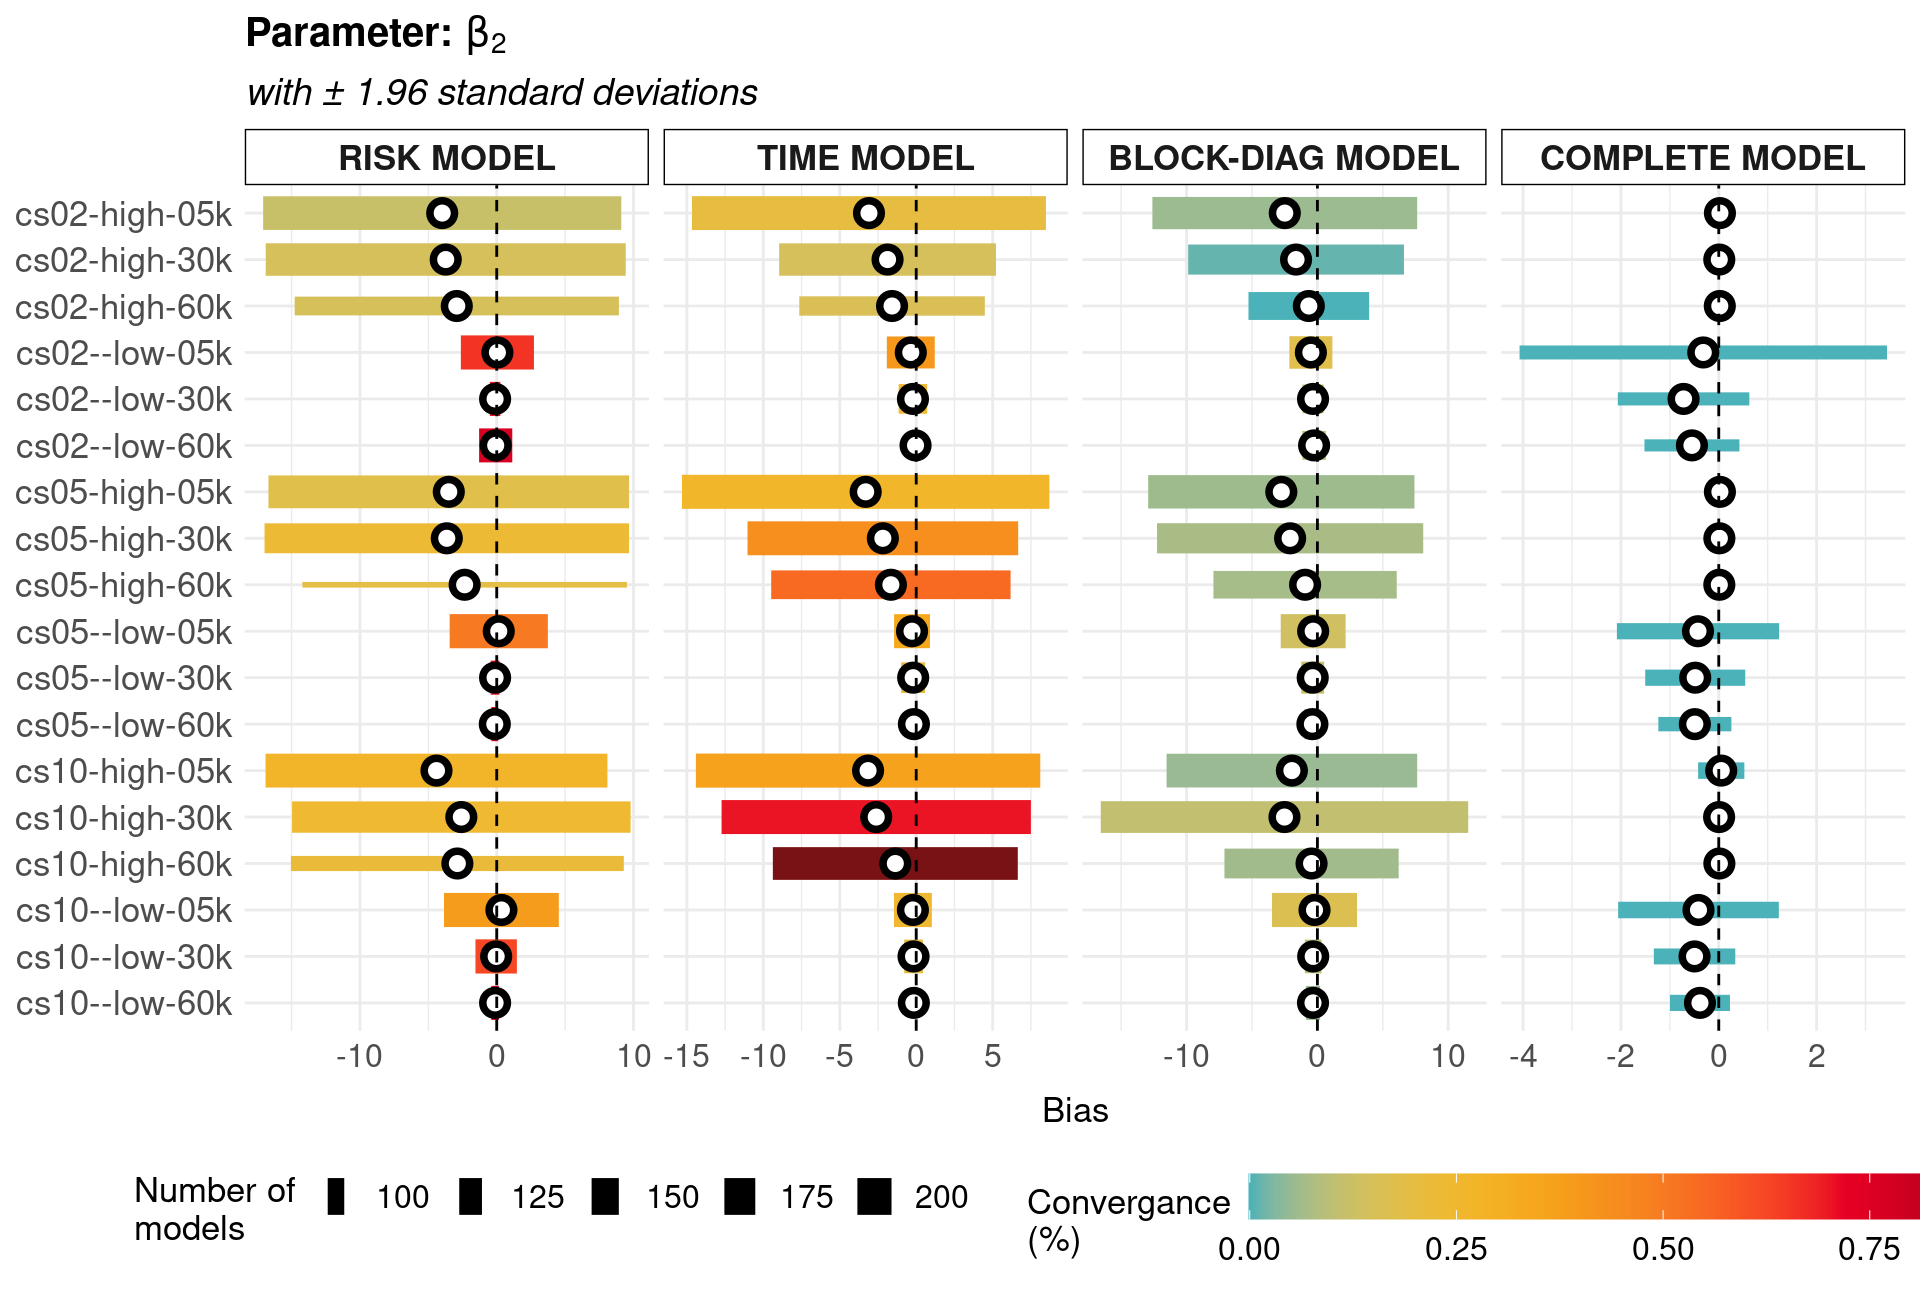
\includegraphics[width=\textwidth]{bias2plotsd-2.png}\\
 \begin{footnotesize}
  SOURCE: The author (2021).
 \end{footnotesize}
 \label{fig:biassdbeta2}
\end{figure}

\begin{figure}[H]
 \setlength{\abovecaptionskip}{.0001pt}
 \caption{PARAMETER \(\gamma_{1}\) BIAS WITH \(\pm\) 1.96 STANDARD
          DEVIATIONS}
 \vspace{0.2cm}\centering
 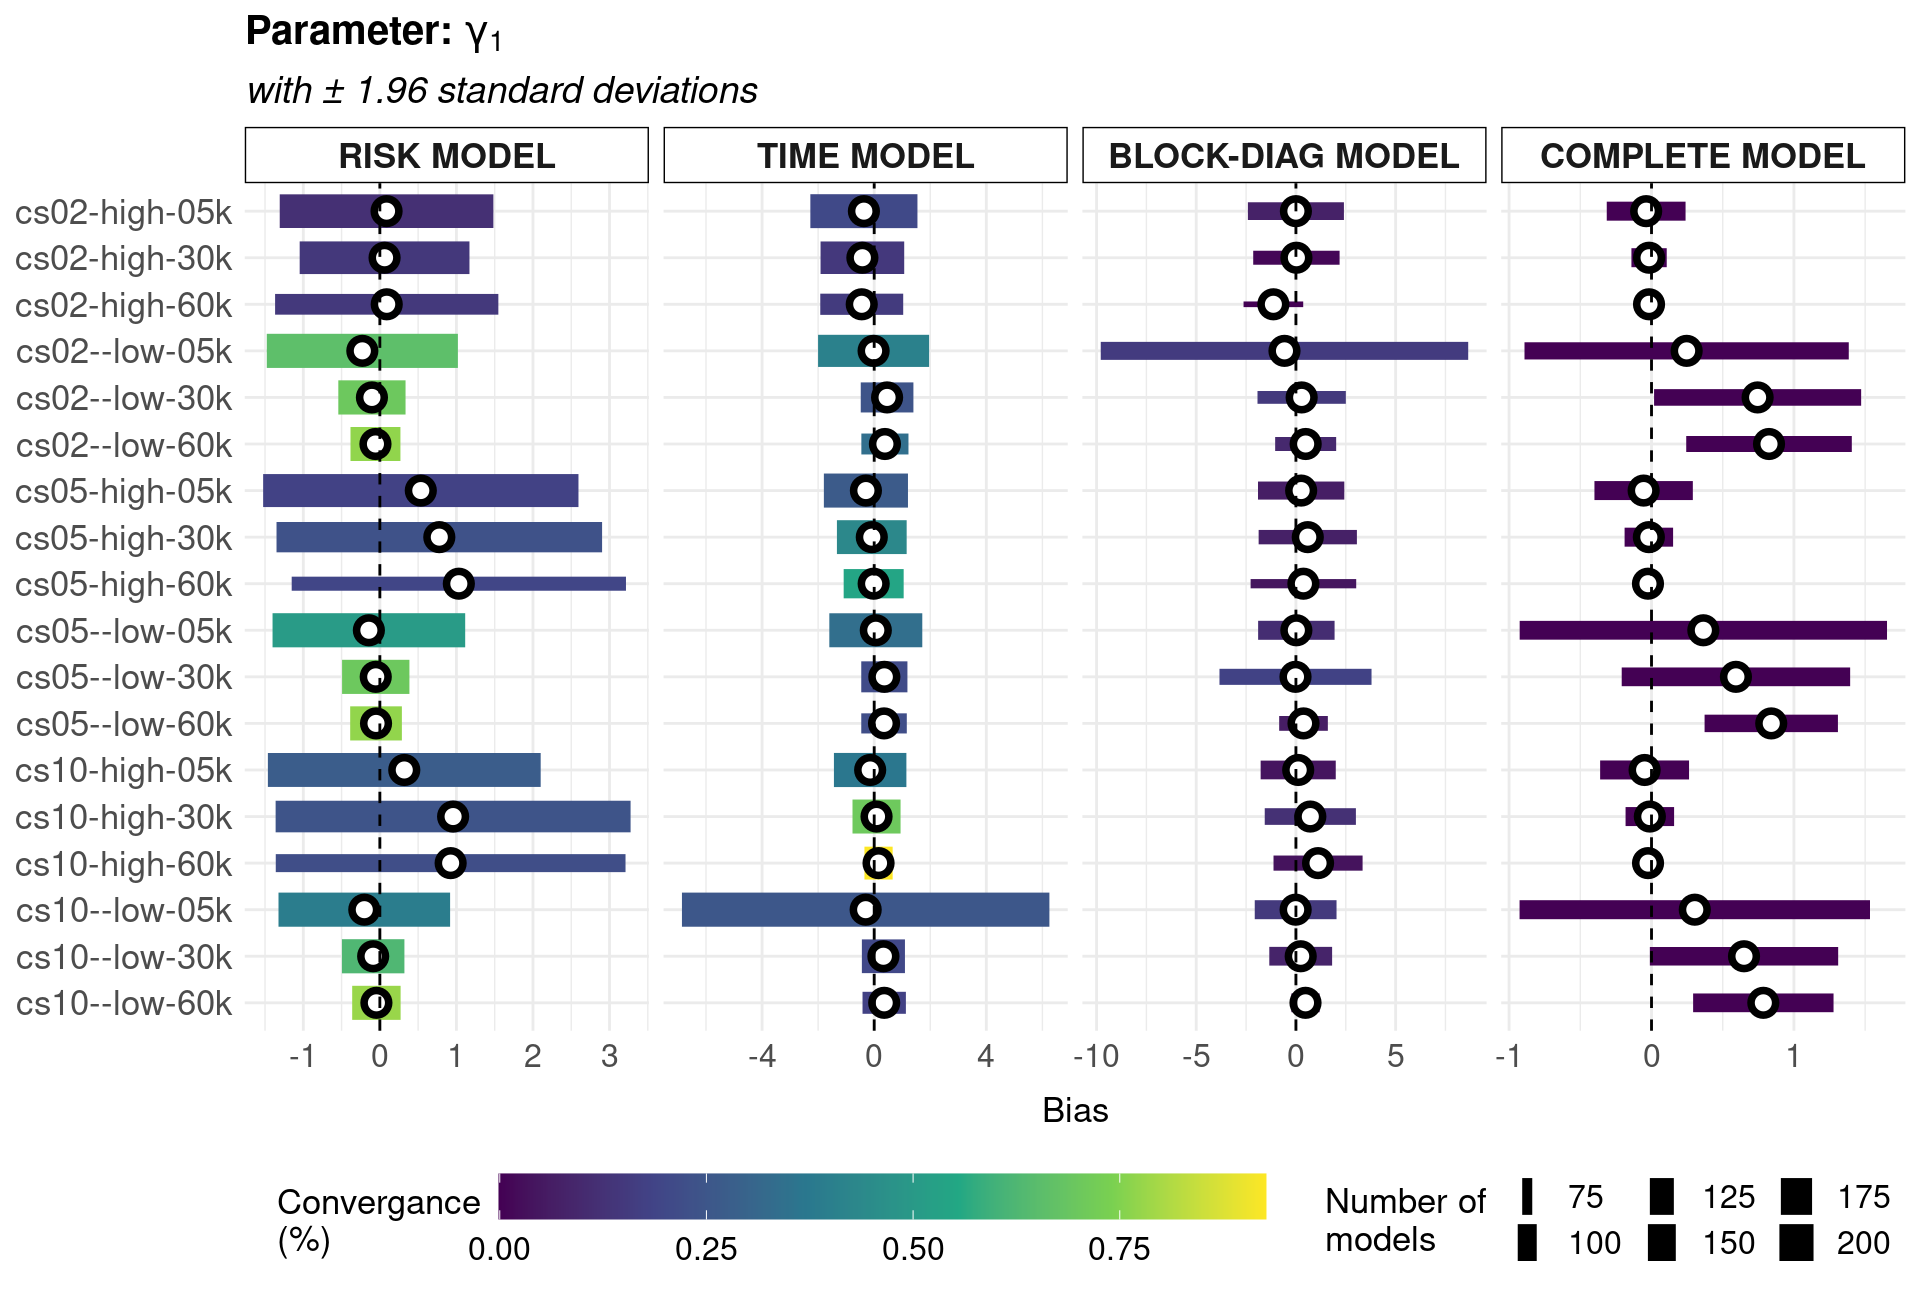
\includegraphics[width=\textwidth]{bias2plotsd-3.png}\\
 \begin{footnotesize}
  SOURCE: The author (2021).
 \end{footnotesize}
 \label{fig:biassdgama1}
\end{figure}

\begin{figure}[H]
 \setlength{\abovecaptionskip}{.0001pt}
 \caption{PARAMETER \(\gamma_{2}\) BIAS WITH \(\pm\) 1.96 STANDARD
          DEVIATIONS}
 \vspace{0.2cm}\centering
 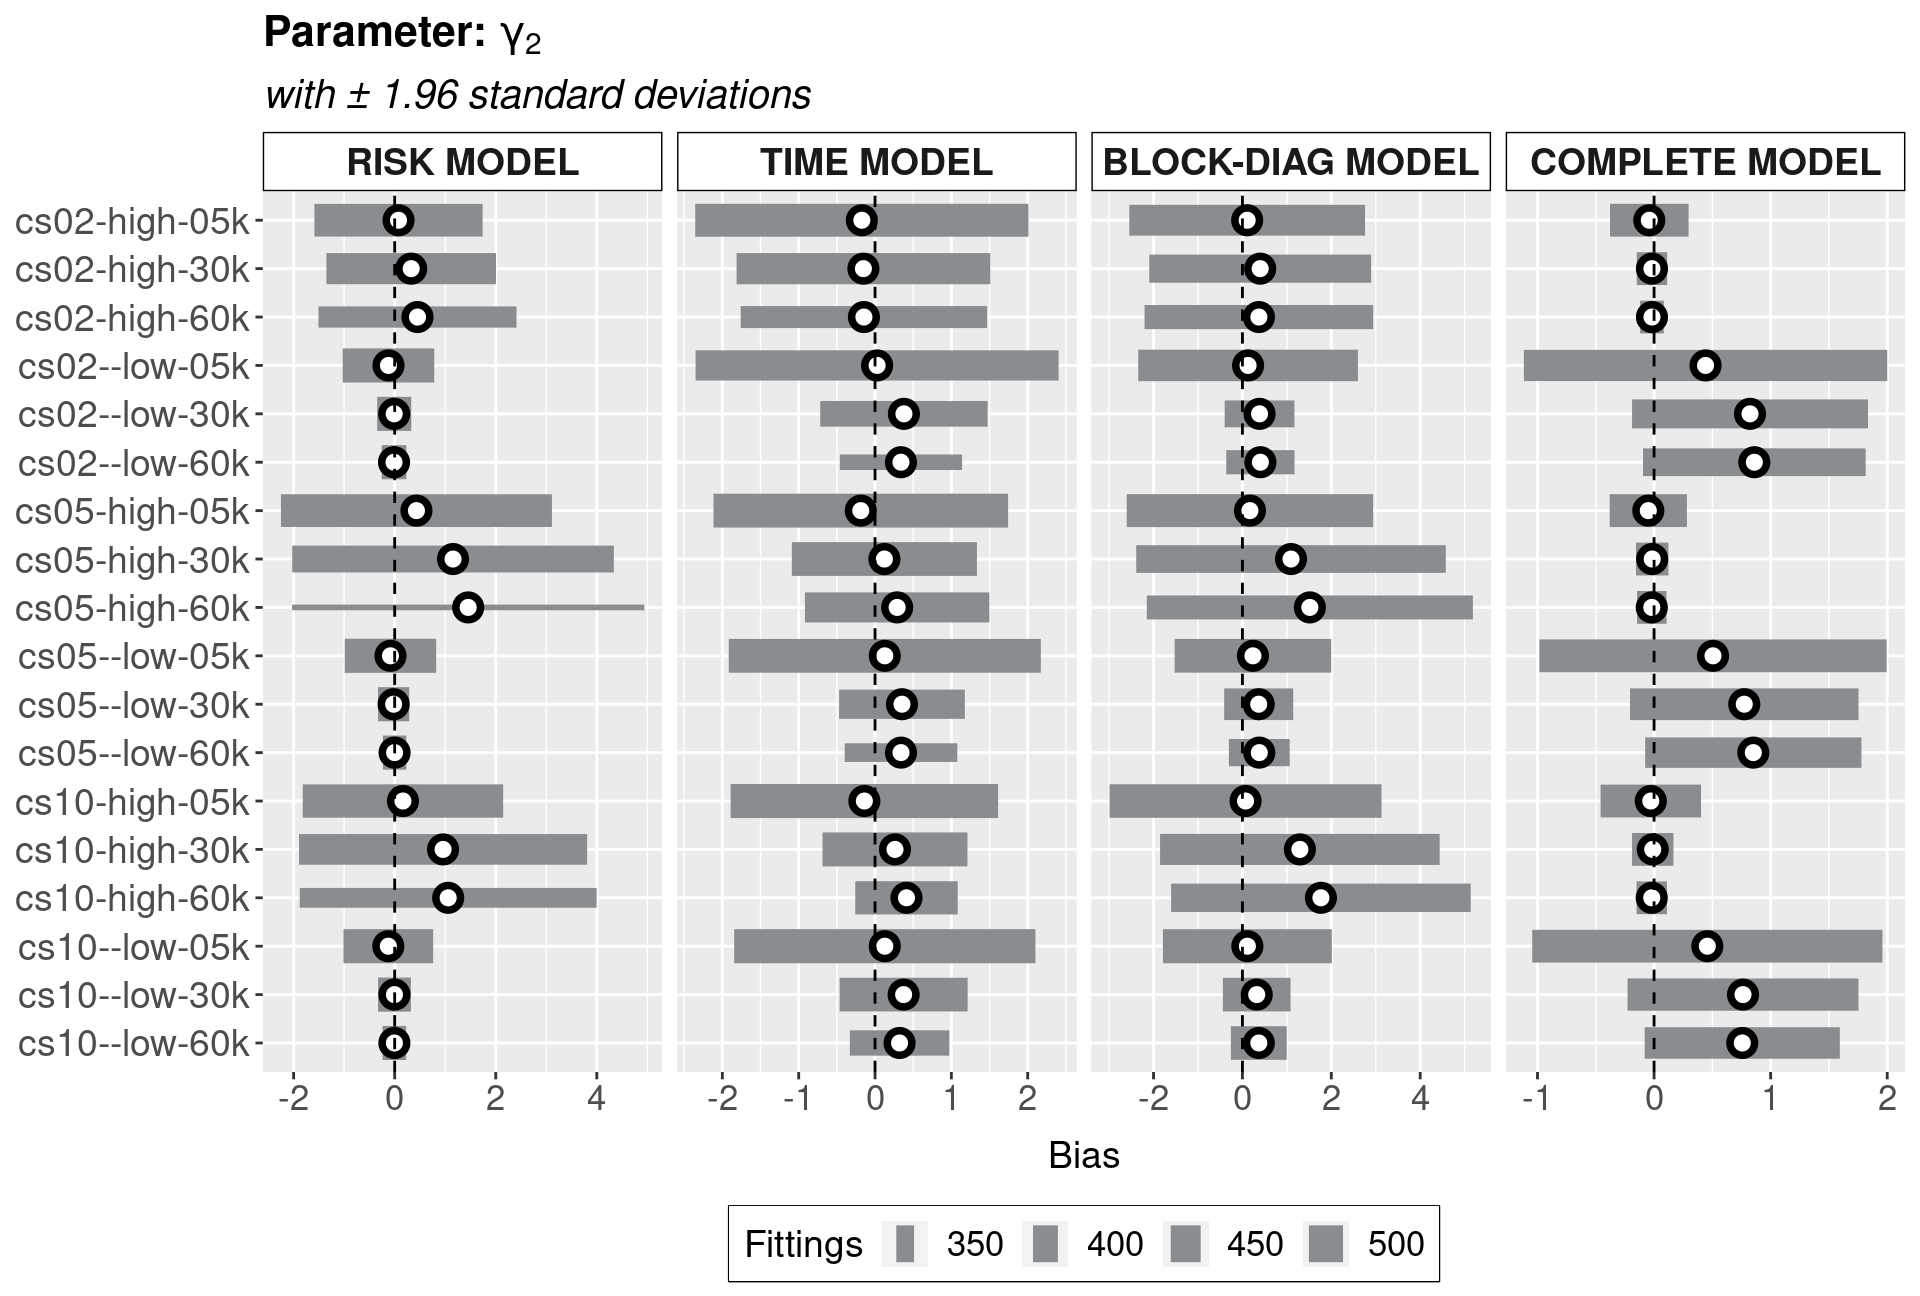
\includegraphics[width=\textwidth]{bias2plotsd-4.png}\\
 \begin{footnotesize}
  SOURCE: The author (2021).
 \end{footnotesize}
 \label{fig:biassdgama2}
\end{figure}

\begin{figure}[H]
 \setlength{\abovecaptionskip}{.0001pt}
 \caption{PARAMETER \(w_{1}\) BIAS WITH \(\pm\) 1.96 STANDARD DEVIATIONS}
 \vspace{0.2cm}\centering
 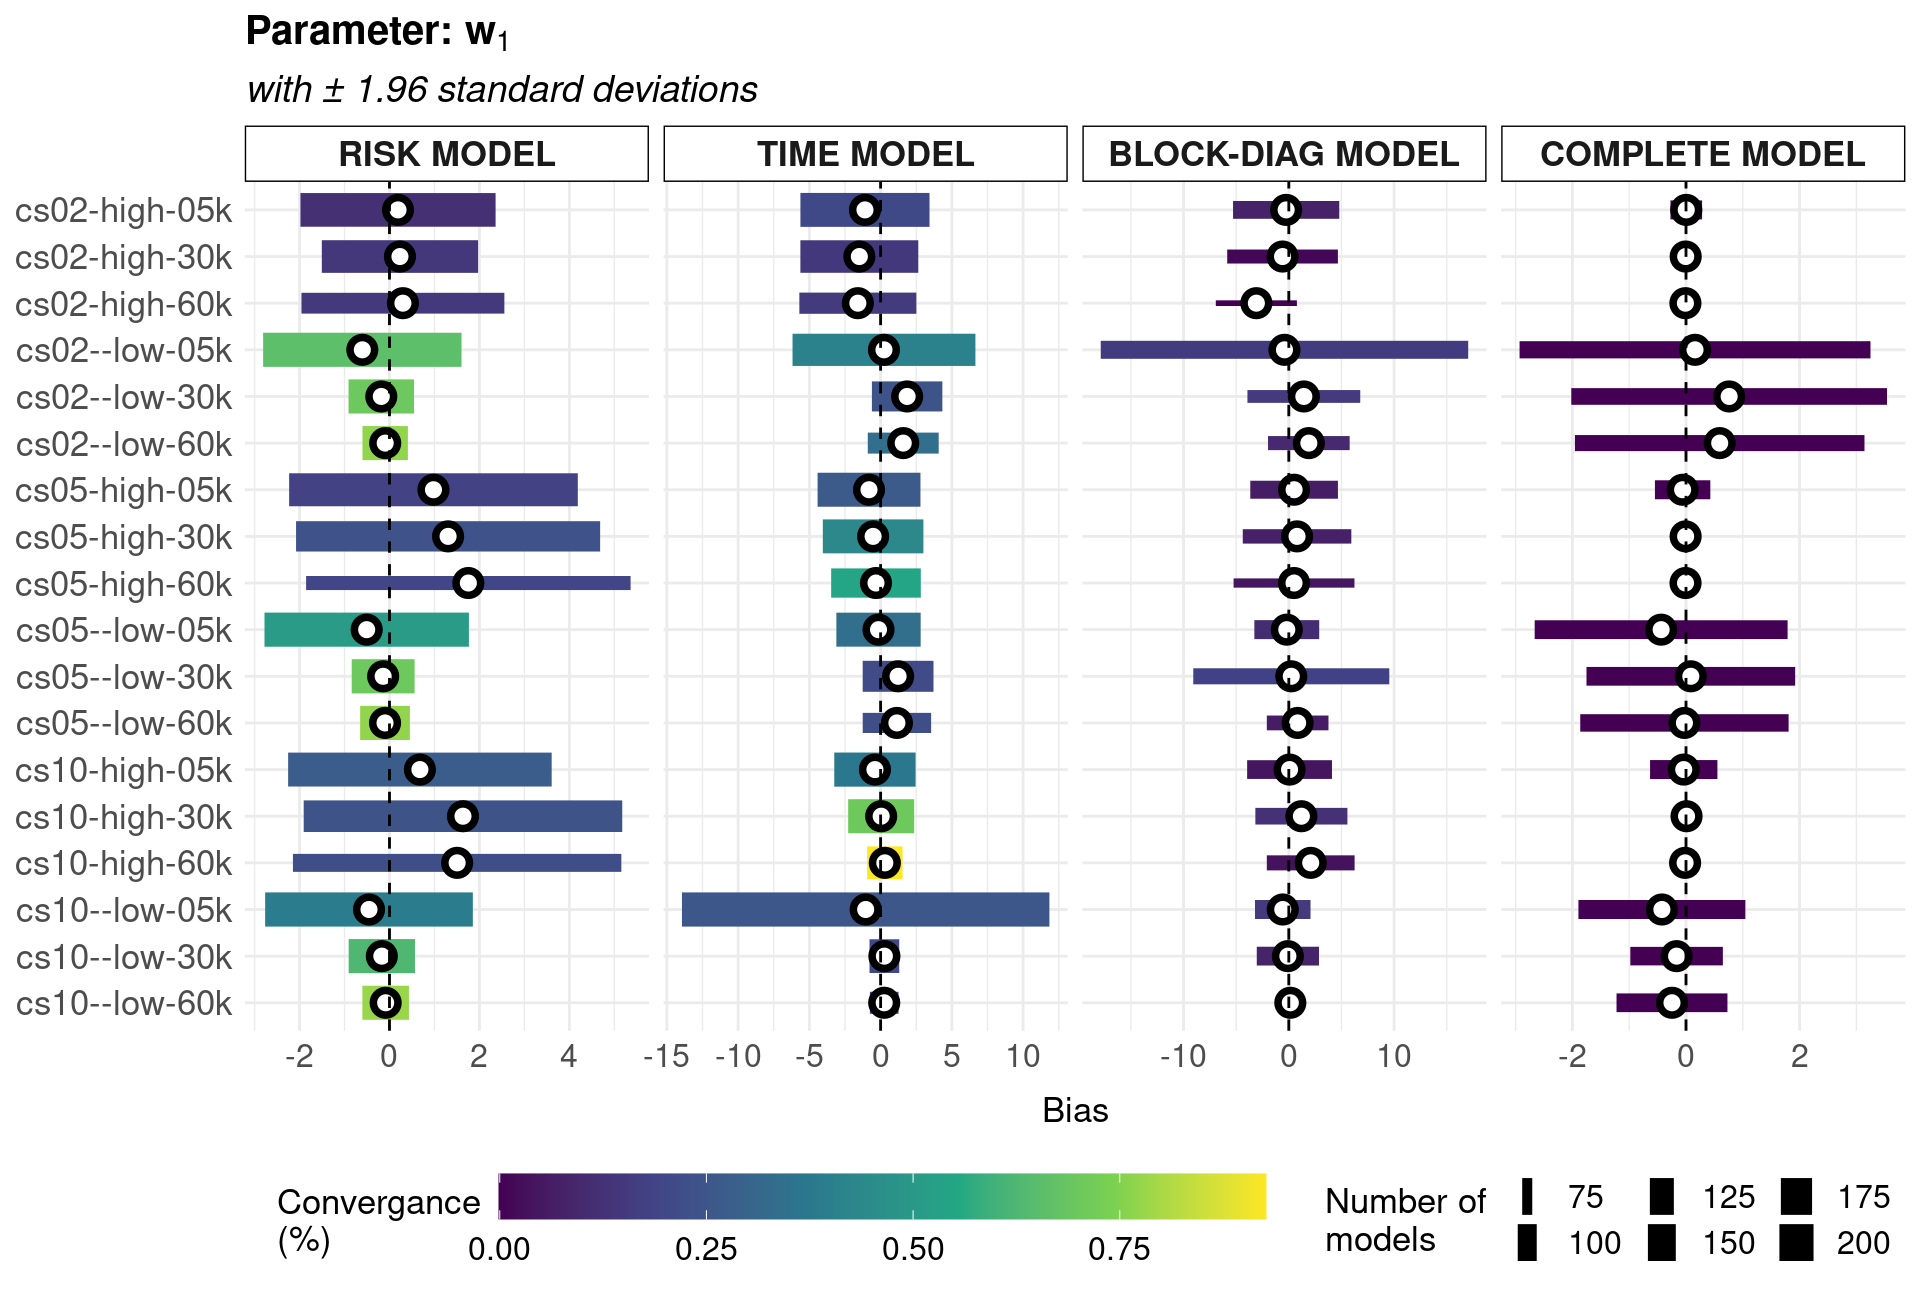
\includegraphics[width=\textwidth]{bias2plotsd-5.png}\\
 \begin{footnotesize}
  SOURCE: The author (2021).
 \end{footnotesize}
 \label{fig:biassdw1}
\end{figure}

\begin{figure}[H]
 \setlength{\abovecaptionskip}{.0001pt}
 \caption{PARAMETER \(w_{2}\) BIAS WITH \(\pm\) 1.96 STANDARD DEVIATIONS}
 \vspace{0.2cm}\centering
 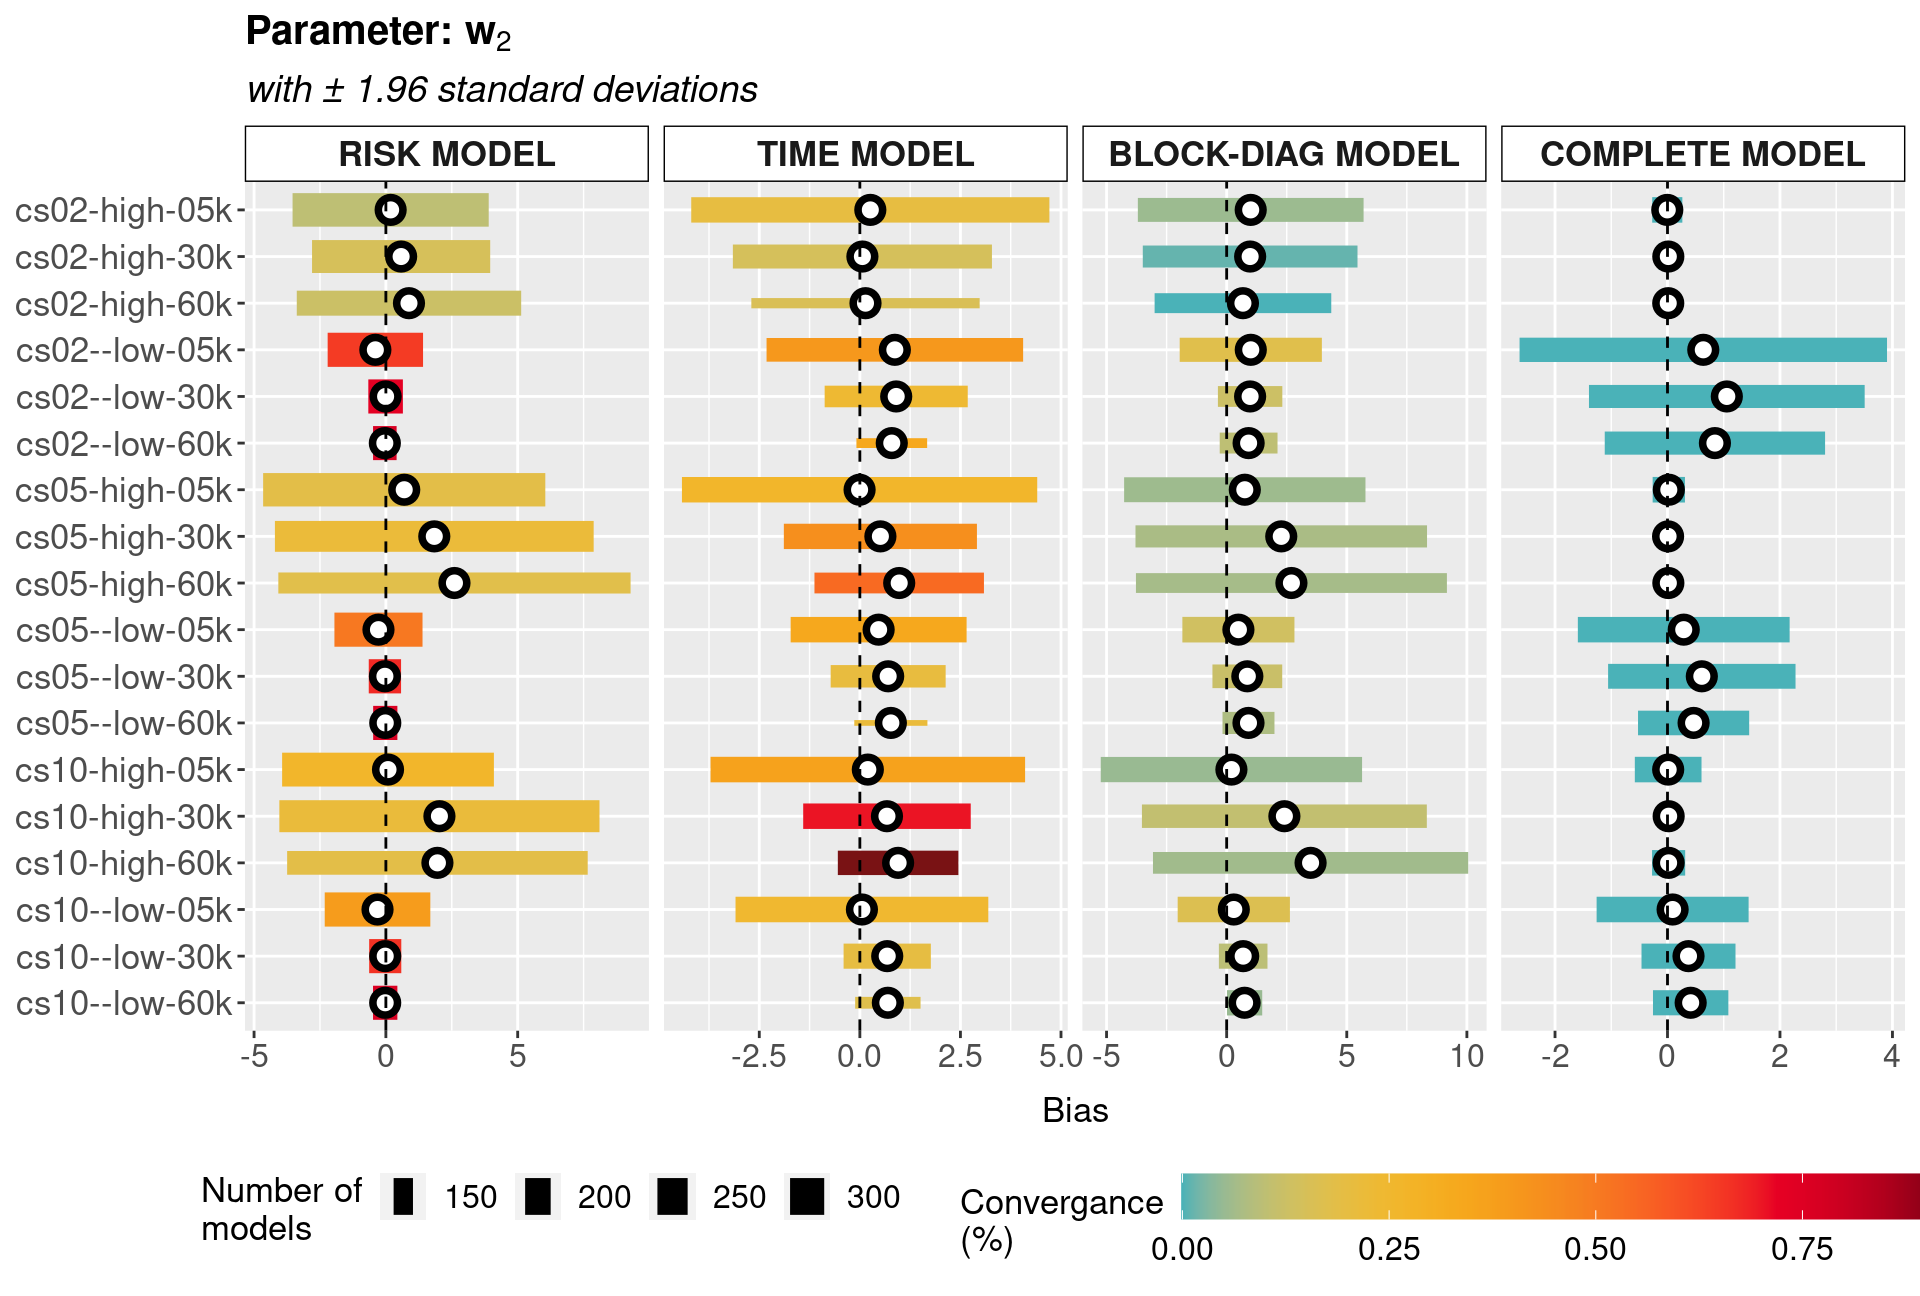
\includegraphics[width=\textwidth]{bias2plotsd-6.png}\\
 \begin{footnotesize}
  SOURCE: The author (2021).
 \end{footnotesize}
 \label{fig:biassdw2}
\end{figure}

\begin{figure}[H]
 \setlength{\abovecaptionskip}{.0001pt}
 \caption{PARAMETER \(\log(\sigma_{1}^{2})\) BIAS WITH \(\pm\) 1.96
          STANDARD DEVIATIONS}
 \vspace{0.2cm}\centering
 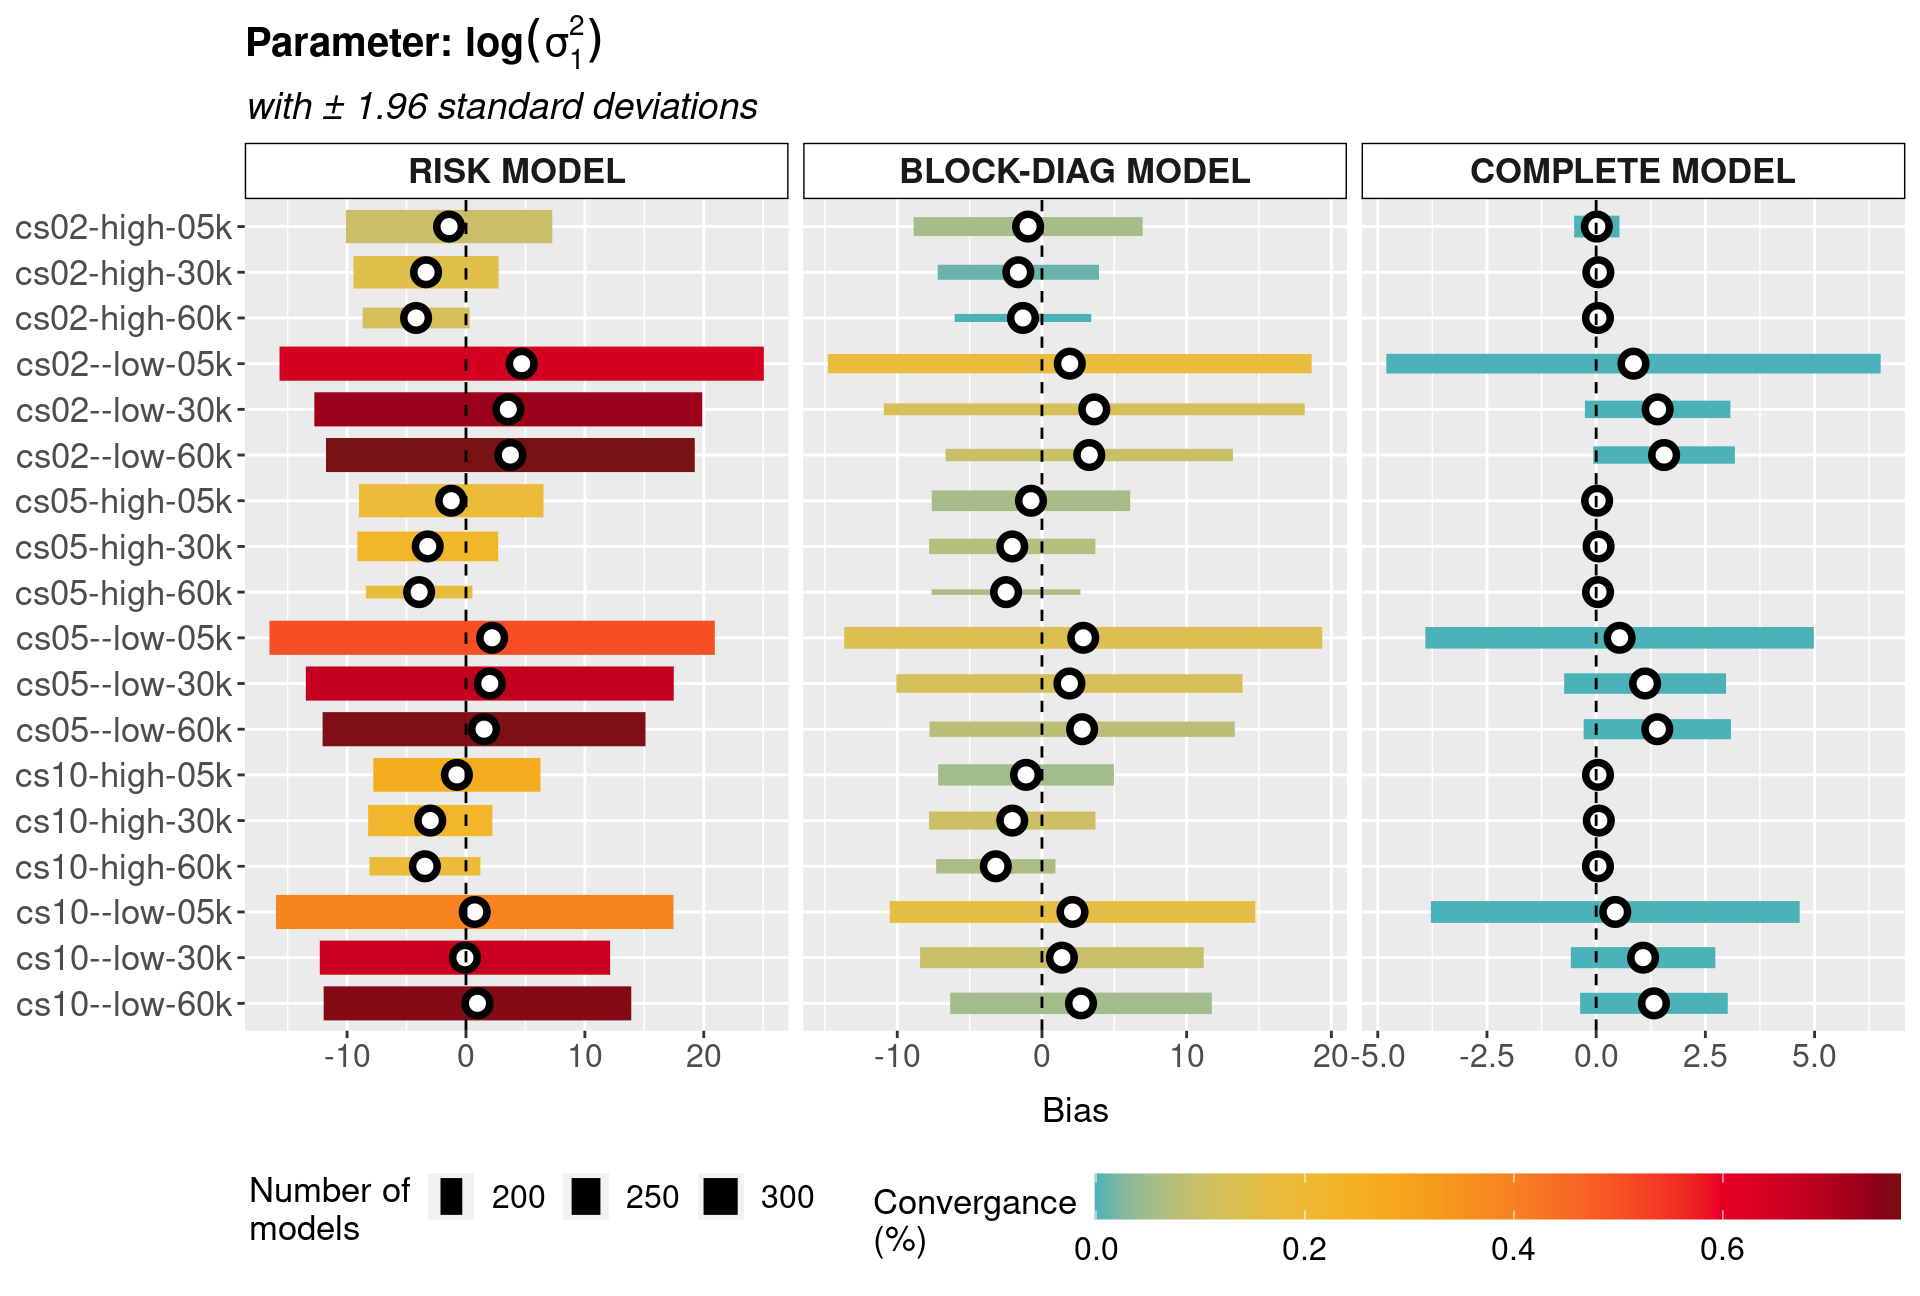
\includegraphics[width=\textwidth]{bias2plotsd-7.png}\\
 \begin{footnotesize}
  SOURCE: The author (2021).
 \end{footnotesize}
 \label{fig:biassdlogs2_1}
\end{figure}

\begin{figure}[H]
 \setlength{\abovecaptionskip}{.0001pt}
 \caption{PARAMETER \(\log(\sigma_{2}^{2})\) BIAS WITH \(\pm\) 1.96
          STANDARD DEVIATIONS}
 \vspace{0.2cm}\centering
 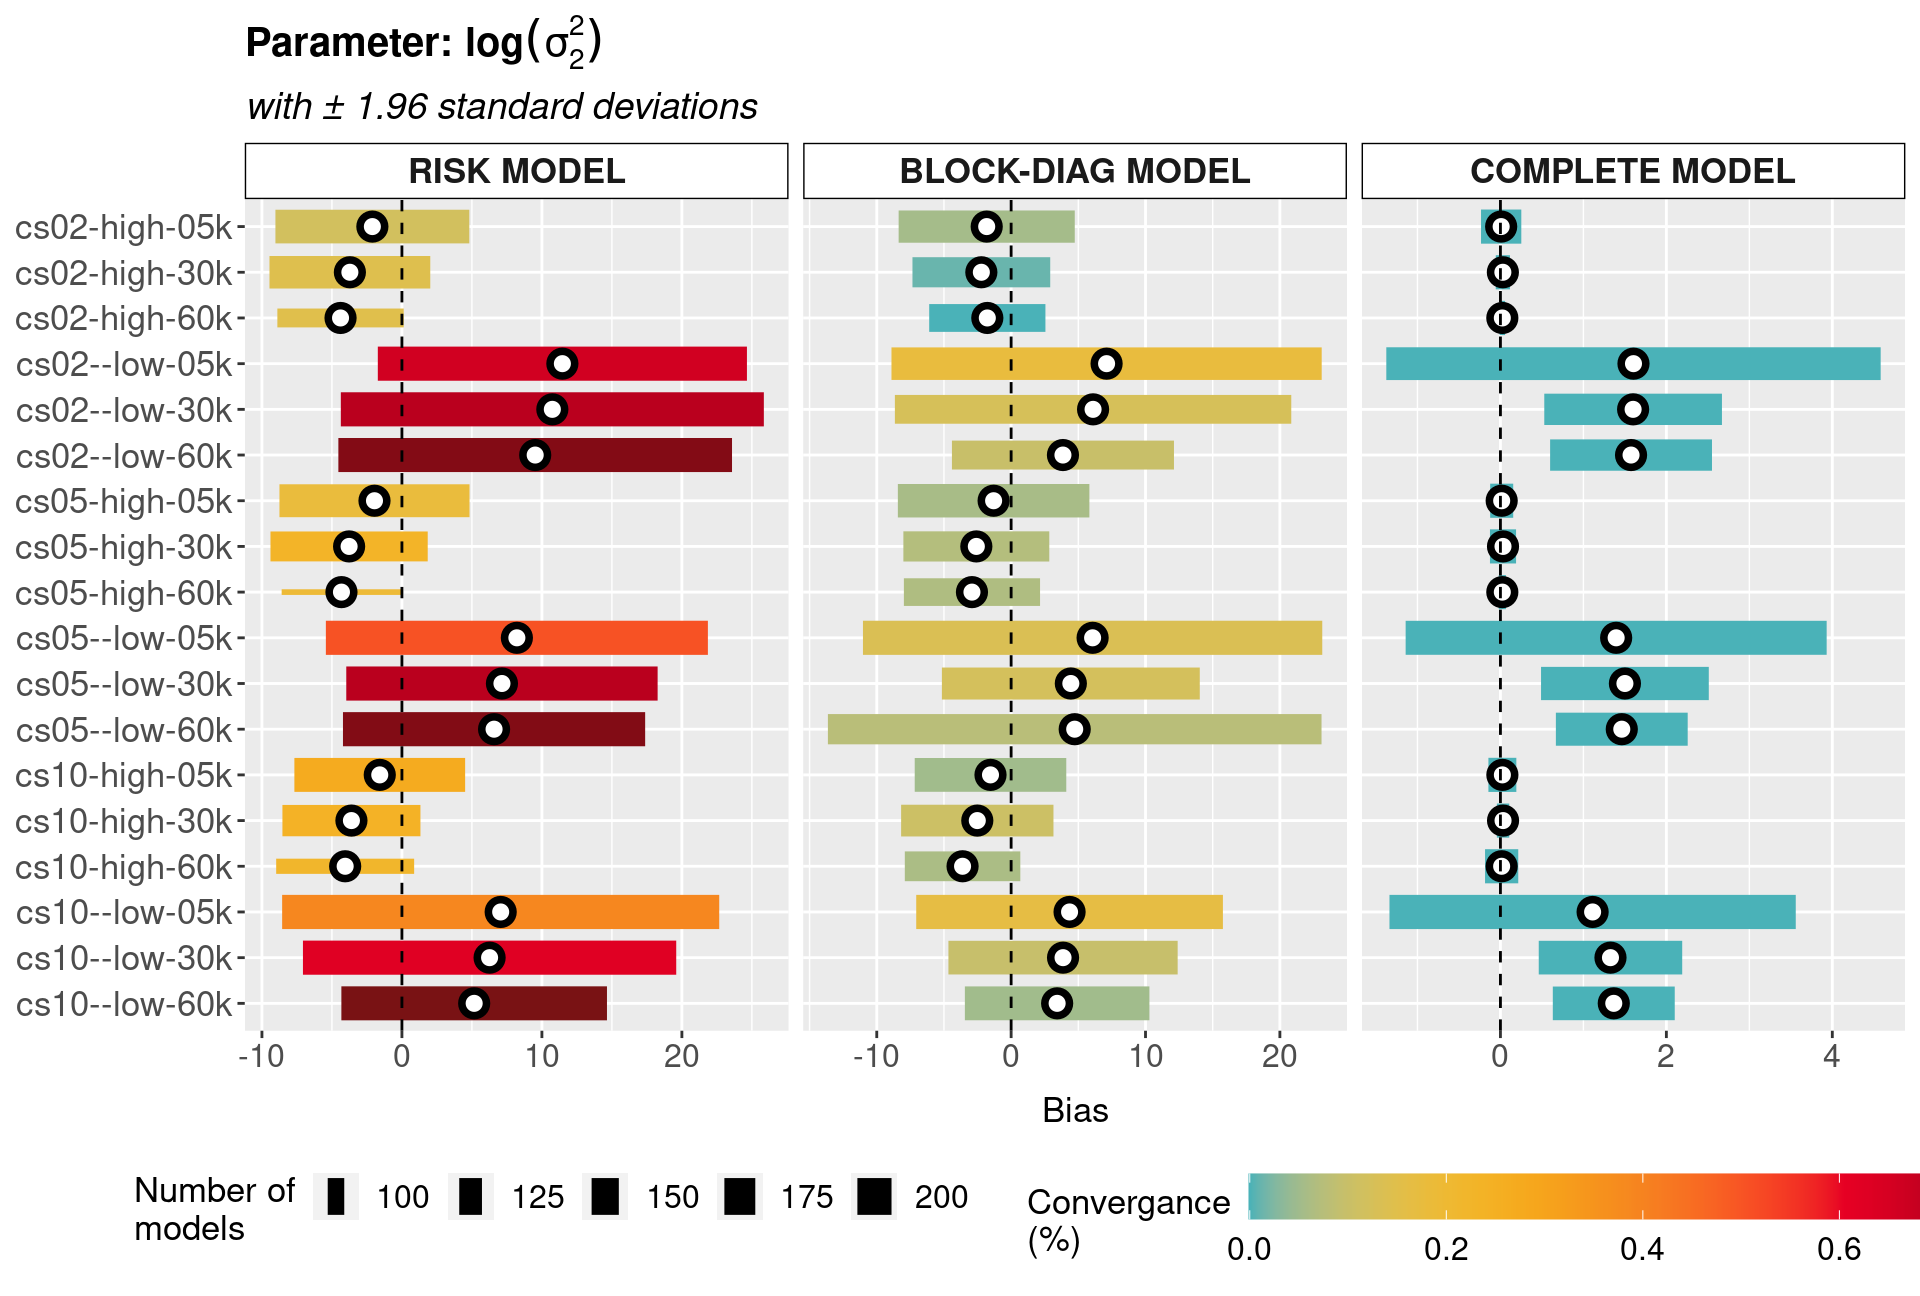
\includegraphics[width=\textwidth]{bias2plotsd-8.png}\\
 \begin{footnotesize}
  SOURCE: The author (2021).
 \end{footnotesize}
 \label{fig:biassdlogs2_2}
\end{figure}

\begin{figure}[H]
 \setlength{\abovecaptionskip}{.0001pt}
 \caption{PARAMETER \(\log(\sigma_{3}^{2})\) BIAS WITH \(\pm\) 1.96
          STANDARD DEVIATIONS}
 \vspace{0.2cm}\centering
 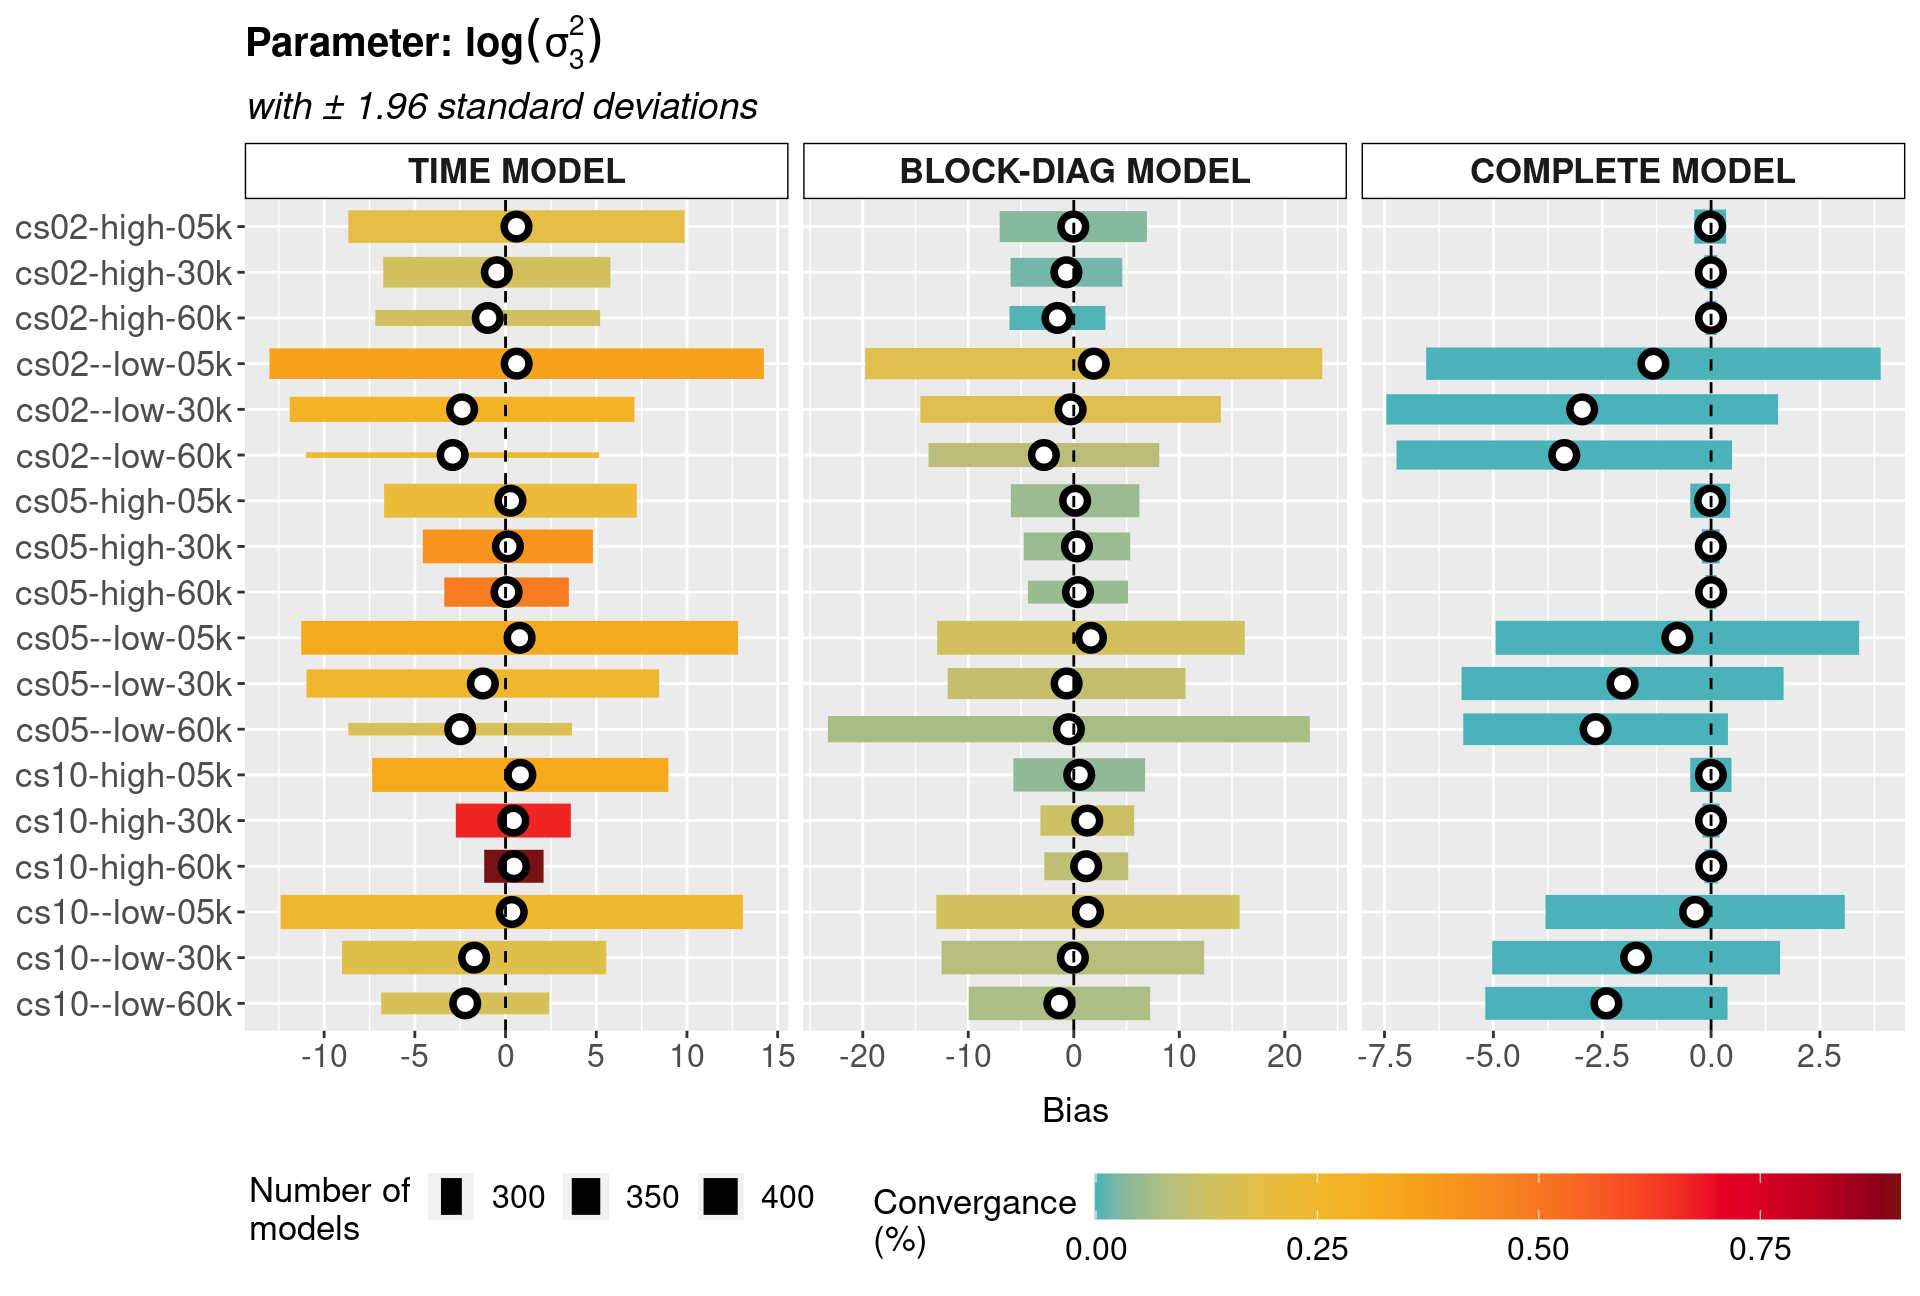
\includegraphics[width=\textwidth]{bias2plotsd-9.png}\\
 \begin{footnotesize}
  SOURCE: The author (2021).
 \end{footnotesize}
 \label{fig:biassdlogs2_3}
\end{figure}

\begin{figure}[H]
 \setlength{\abovecaptionskip}{.0001pt}
 \caption{PARAMETER \(\log(\sigma_{4}^{2})\) BIAS WITH \(\pm\) 1.96
          STANDARD DEVIATIONS}
 \vspace{0.2cm}\centering
 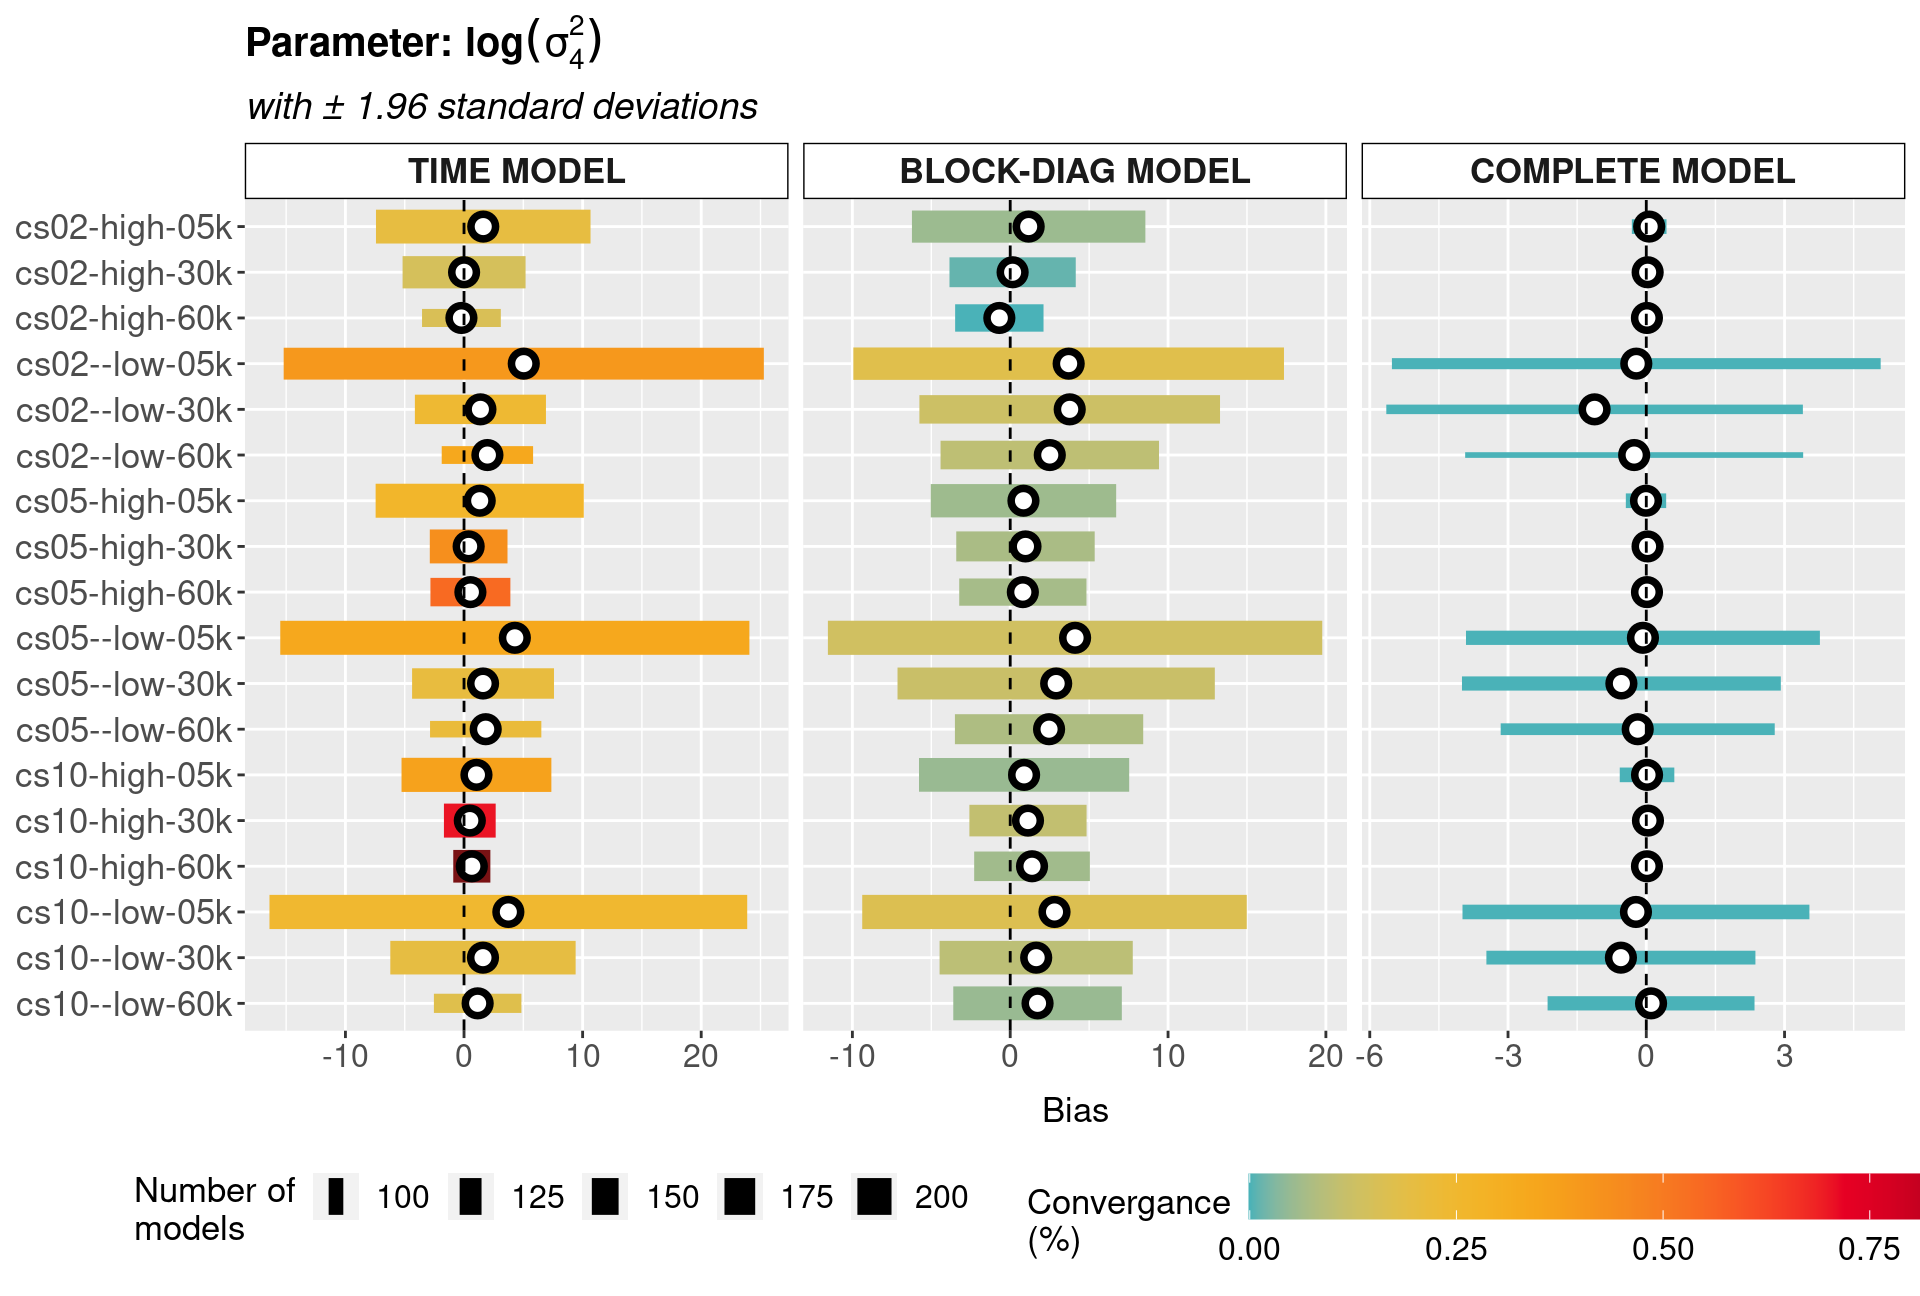
\includegraphics[width=\textwidth]{bias2plotsd-10.png}\\
 \begin{footnotesize}
  SOURCE: The author (2021).
 \end{footnotesize}
 \label{fig:biassdlogs2_4}
\end{figure}

\begin{figure}[H]
 \setlength{\abovecaptionskip}{.0001pt}
 \caption{PARAMETER \(z(\rho_{12})\) BIAS WITH \(\pm\) 1.96 STANDARD
          DEVIATIONS}
 \vspace{0.2cm}\centering
 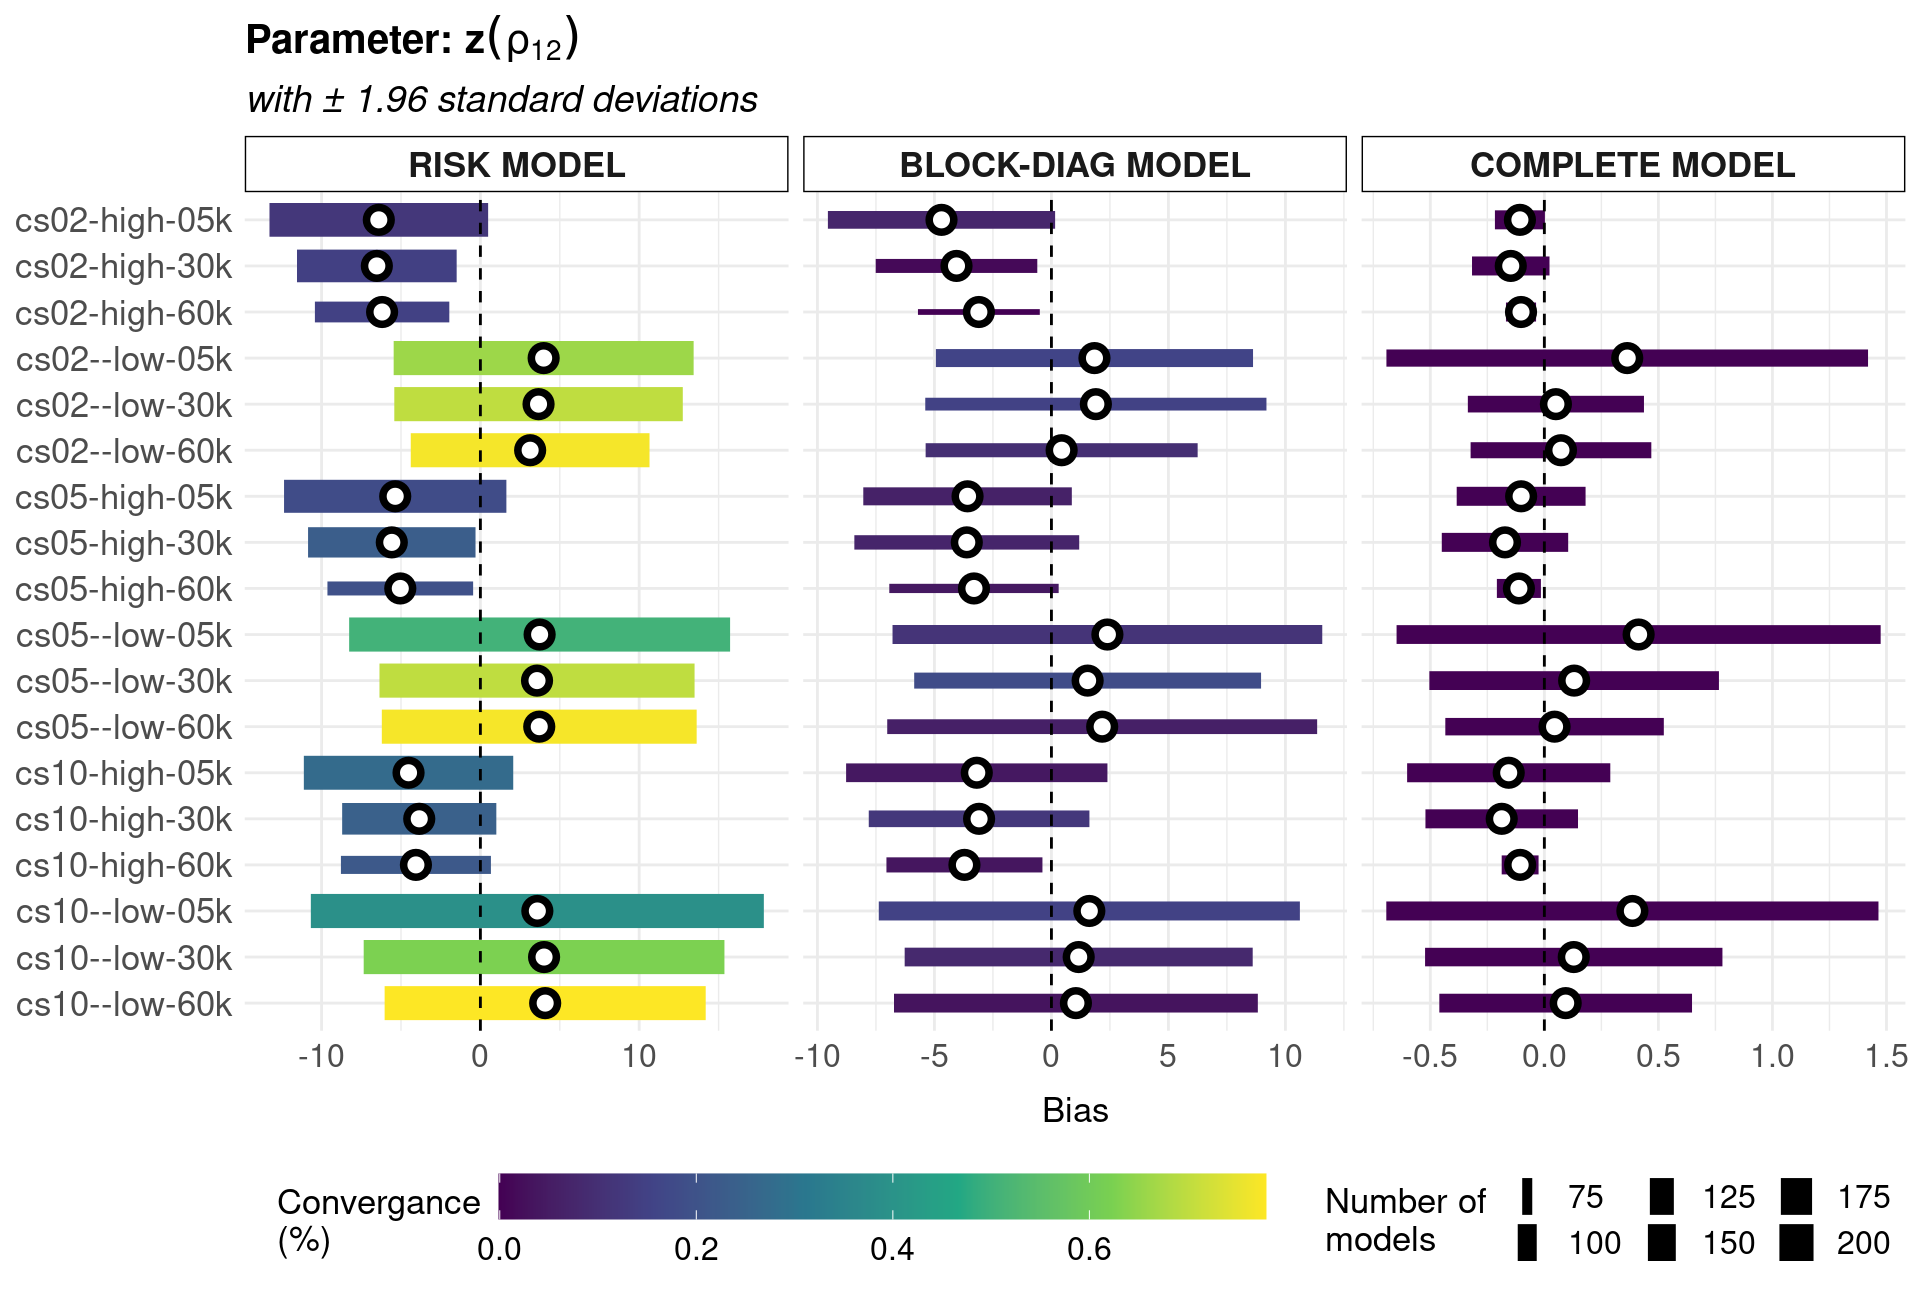
\includegraphics[width=\textwidth]{bias2plotsd-11.png}\\
 \begin{footnotesize}
  SOURCE: The author (2021).
 \end{footnotesize}
 \label{fig:biassdrhoz12}
\end{figure}

\begin{figure}[H]
 \setlength{\abovecaptionskip}{.0001pt}
 \caption{PARAMETER \(z(\rho_{34})\) BIAS WITH \(\pm\) 1.96 STANDARD
          DEVIATIONS}
 \vspace{0.2cm}\centering
 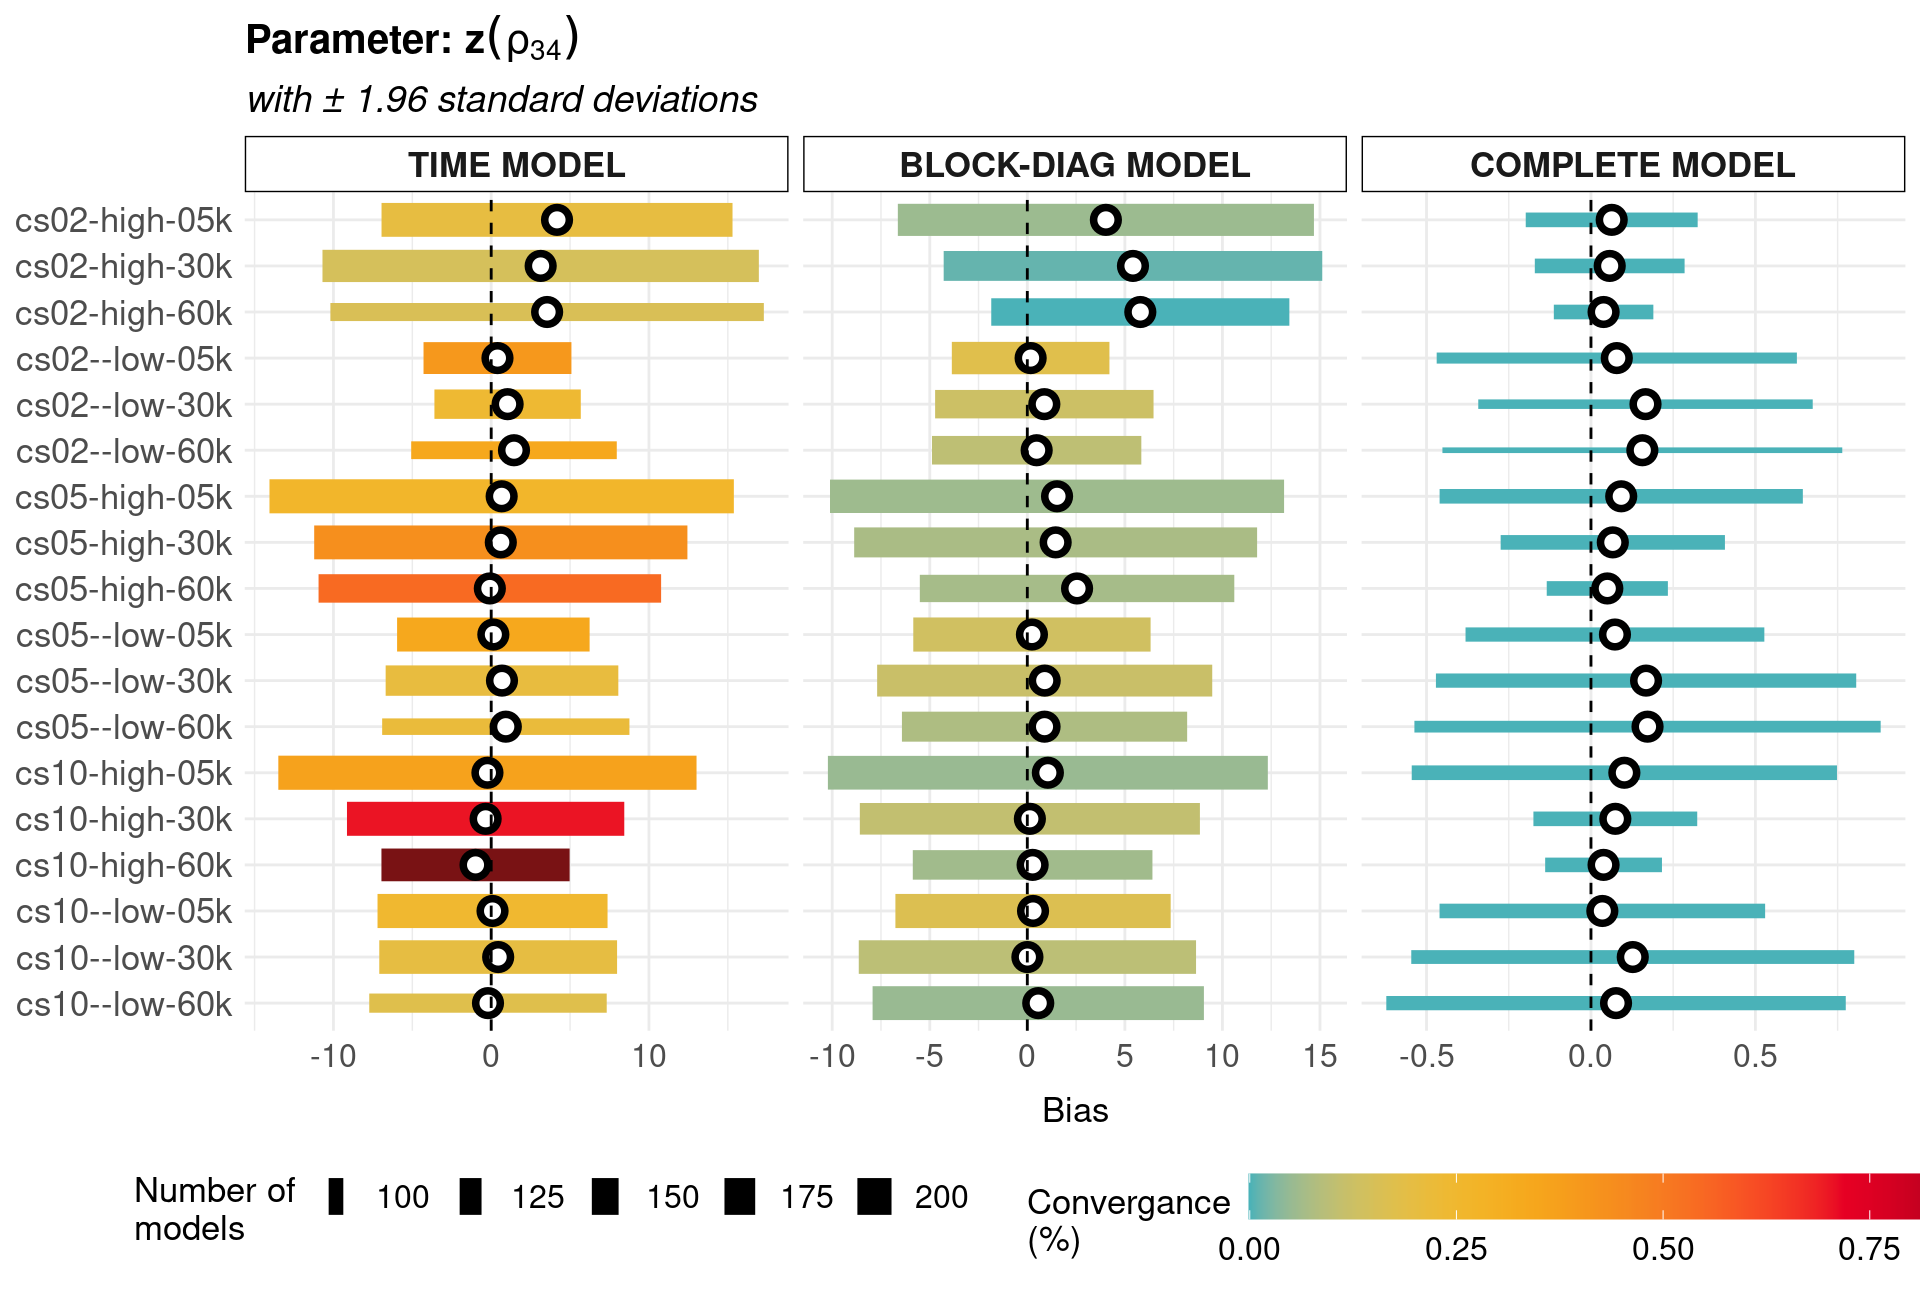
\includegraphics[width=\textwidth]{bias2plotsd-12.png}\\
 \begin{footnotesize}
  SOURCE: The author (2021).
 \end{footnotesize}
 \label{fig:biassdrhoz34}
\end{figure}

\begin{figure}[H]
 \setlength{\abovecaptionskip}{.0001pt}
 \caption{PARAMETERS
          \(\{z(\rho_{13}),~z(\rho_{24}),~z(\rho_{14}),~z(\rho_{23})\}\)
          BIAS WITH \(\pm\) 1.96 STANDARD DEVIATIONS}
 \vspace{0.2cm}\centering
 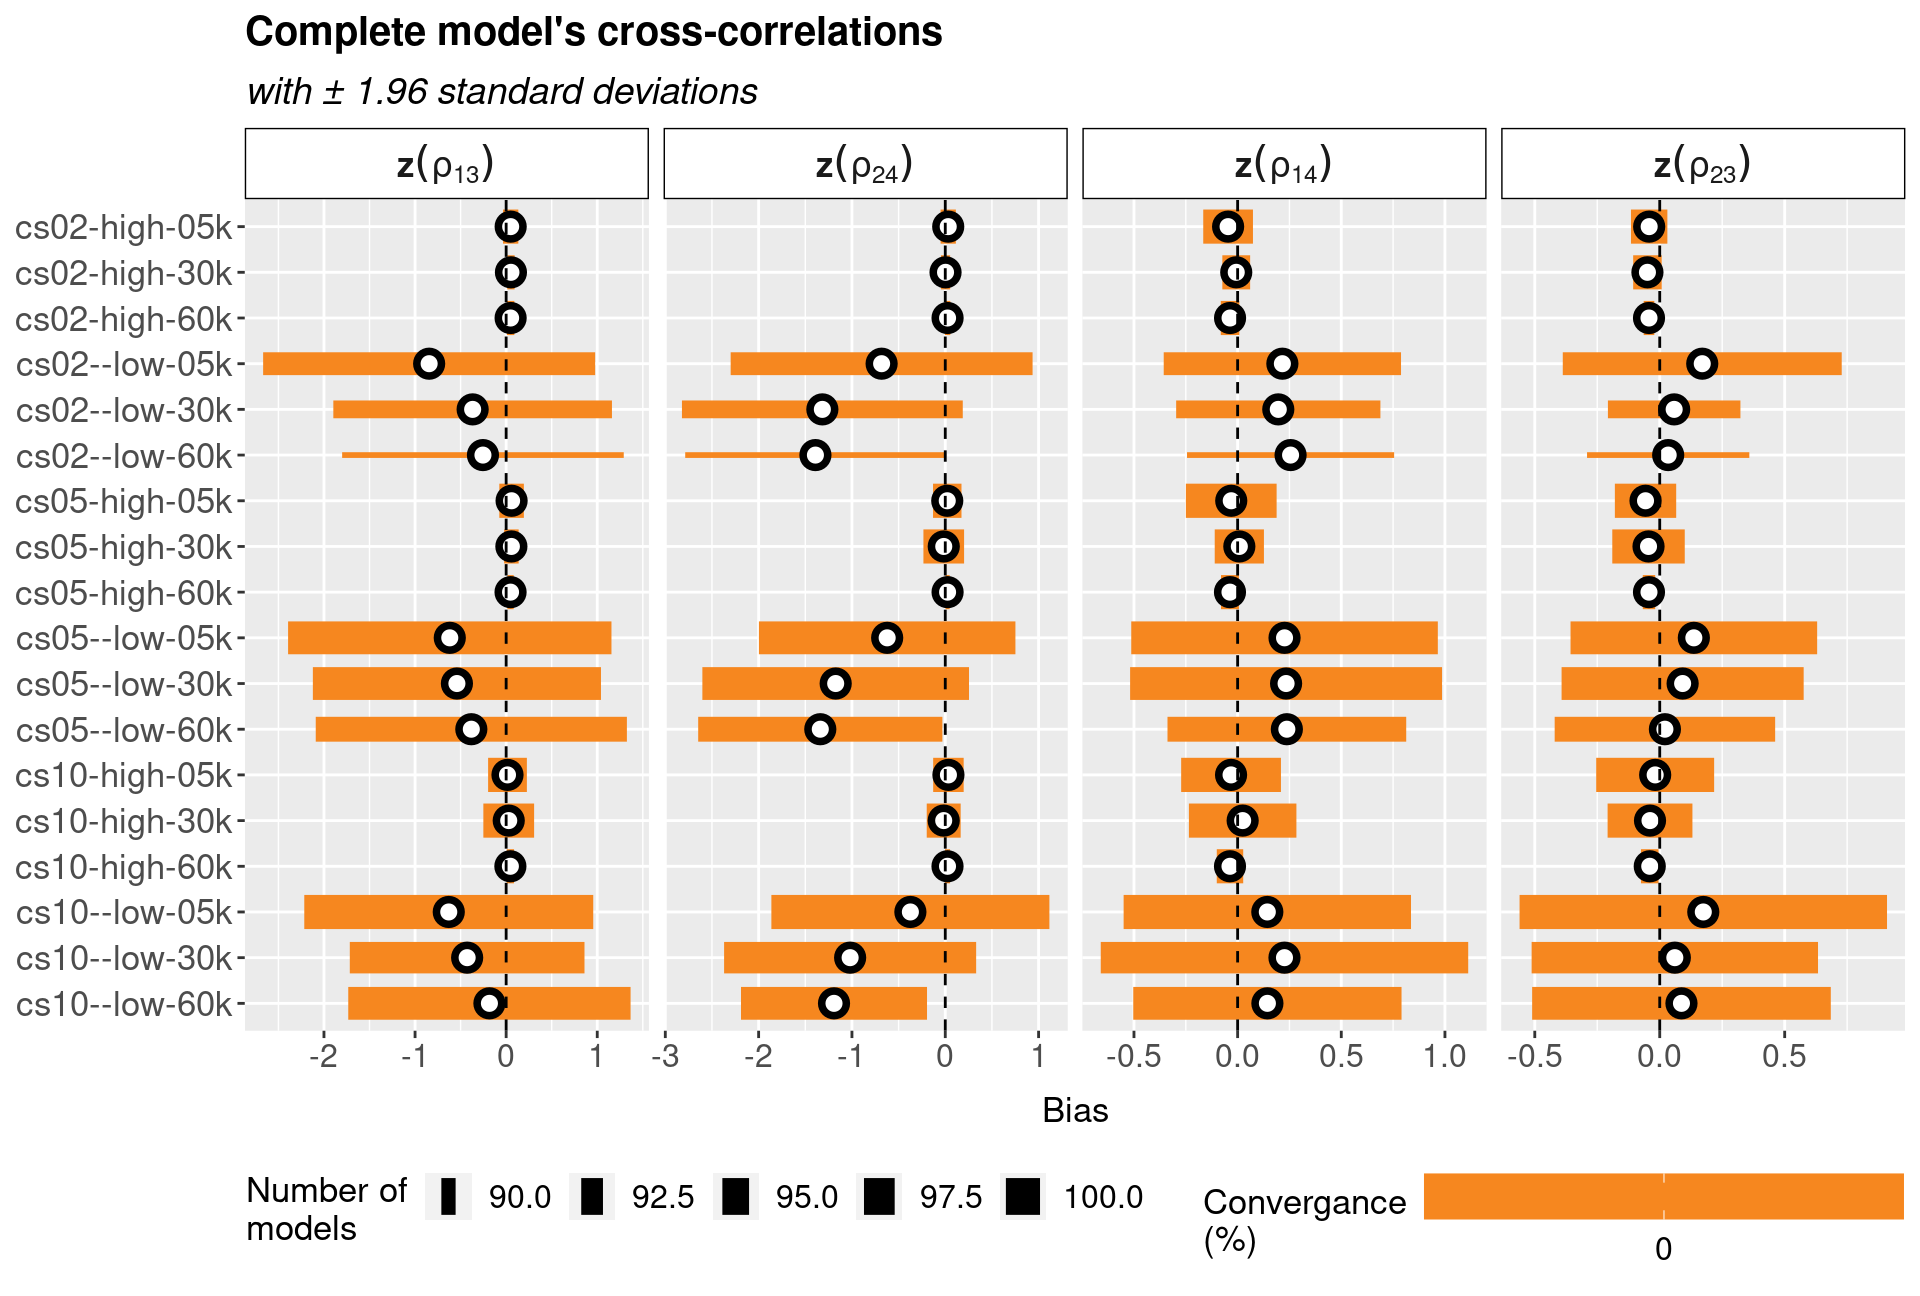
\includegraphics[width=\textwidth]{bias2plotsd-13.png}\\
 \begin{footnotesize}
  SOURCE: The author (2021).
 \end{footnotesize}
 \label{fig:biassdrhoz4}
\end{figure}

In the \textit{simpler} models, with a latent structure just in one
level, is hard to see some significant difference between the clusters
and sample sizes. With the complete model, in the other hand, the
difference is clear: as we increase the clusters and the sample sizes,
the bias-variance decreases. The mean-bias is basically always the
same. In the risk and block-diag models is hard to point-out a scenario
as the best or worst. For the time model, with the scenario of cluster
size 10; low CiF; and 5 thousand data points, we get a much bigger
standard deviation in two of the parameters.

With the log-variances presented in \autoref{fig:biassdlogs2_1},
\autoref{fig:biassdlogs2_2}, \autoref{fig:biassdlogs2_3}, and
\autoref{fig:biassdlogs2_4}, we have instead a similar behavior through
the models. For all the models, the high CIF scenarios are the ones with
a smaller mean and bias-variances. From the risk/time model to the
block-diag model, we do not see a significant improvement in terms of
bias reduction. Such improvement, however, is clear when we look at the
complete model. Again, the magick of considering the cross-correlations.

The same said about the log-variances, can be applied to the risk
correlations in \autoref{fig:biassdrhoz12}, with one addendum: the bias
reduction is even bigger. With the time correlation in
\autoref{fig:biassdrhoz34}, we get the same behavior observed with the
fixed-effect parameters i.e., with the simpler models, the smaller
biases are observed in the low CIF scenarios. However, with the complete
model, we get the opposite. With the cross-correlations in
\autoref{fig:biassdrhoz4}, the mean and bias-variances are much smaller
in the high CIF scenarios.

The biggest bias-variances are obtained in the log-variances. A final
remark to be made is about convergences. With the simpler models, not
all of them work, having in some scenarios (generally the ones with 60
thousand data points) a 50\(\sim\)60\% convergence rate. However, from
this 50\(\sim\)60\%, most reach the ideal gradient-based
convergence. With the complete model is the complete
opposite. Basically, all fits reach a convergence (\(\sim\)100\%
performance) but never is the desired gradient-based convergence.

After looking at the parameter biases, let us take a look at the implied
mean-CIF curves. To nicely accommodate all seventy-two scenarios we
split the curves by level-CIF. In \autoref{fig:cifshigh} we have the
high CIF scenario curves and in \autoref{fig:cifslow} the low CIF
scenario curves.

\begin{figure}[H]
 \setlength{\abovecaptionskip}{.0001pt}
 \caption{HIGH CUMULATIVE INCIDENCE FUNCTION (CIF) SCENARIO CURVES}
 \vspace{0.2cm}\centering
 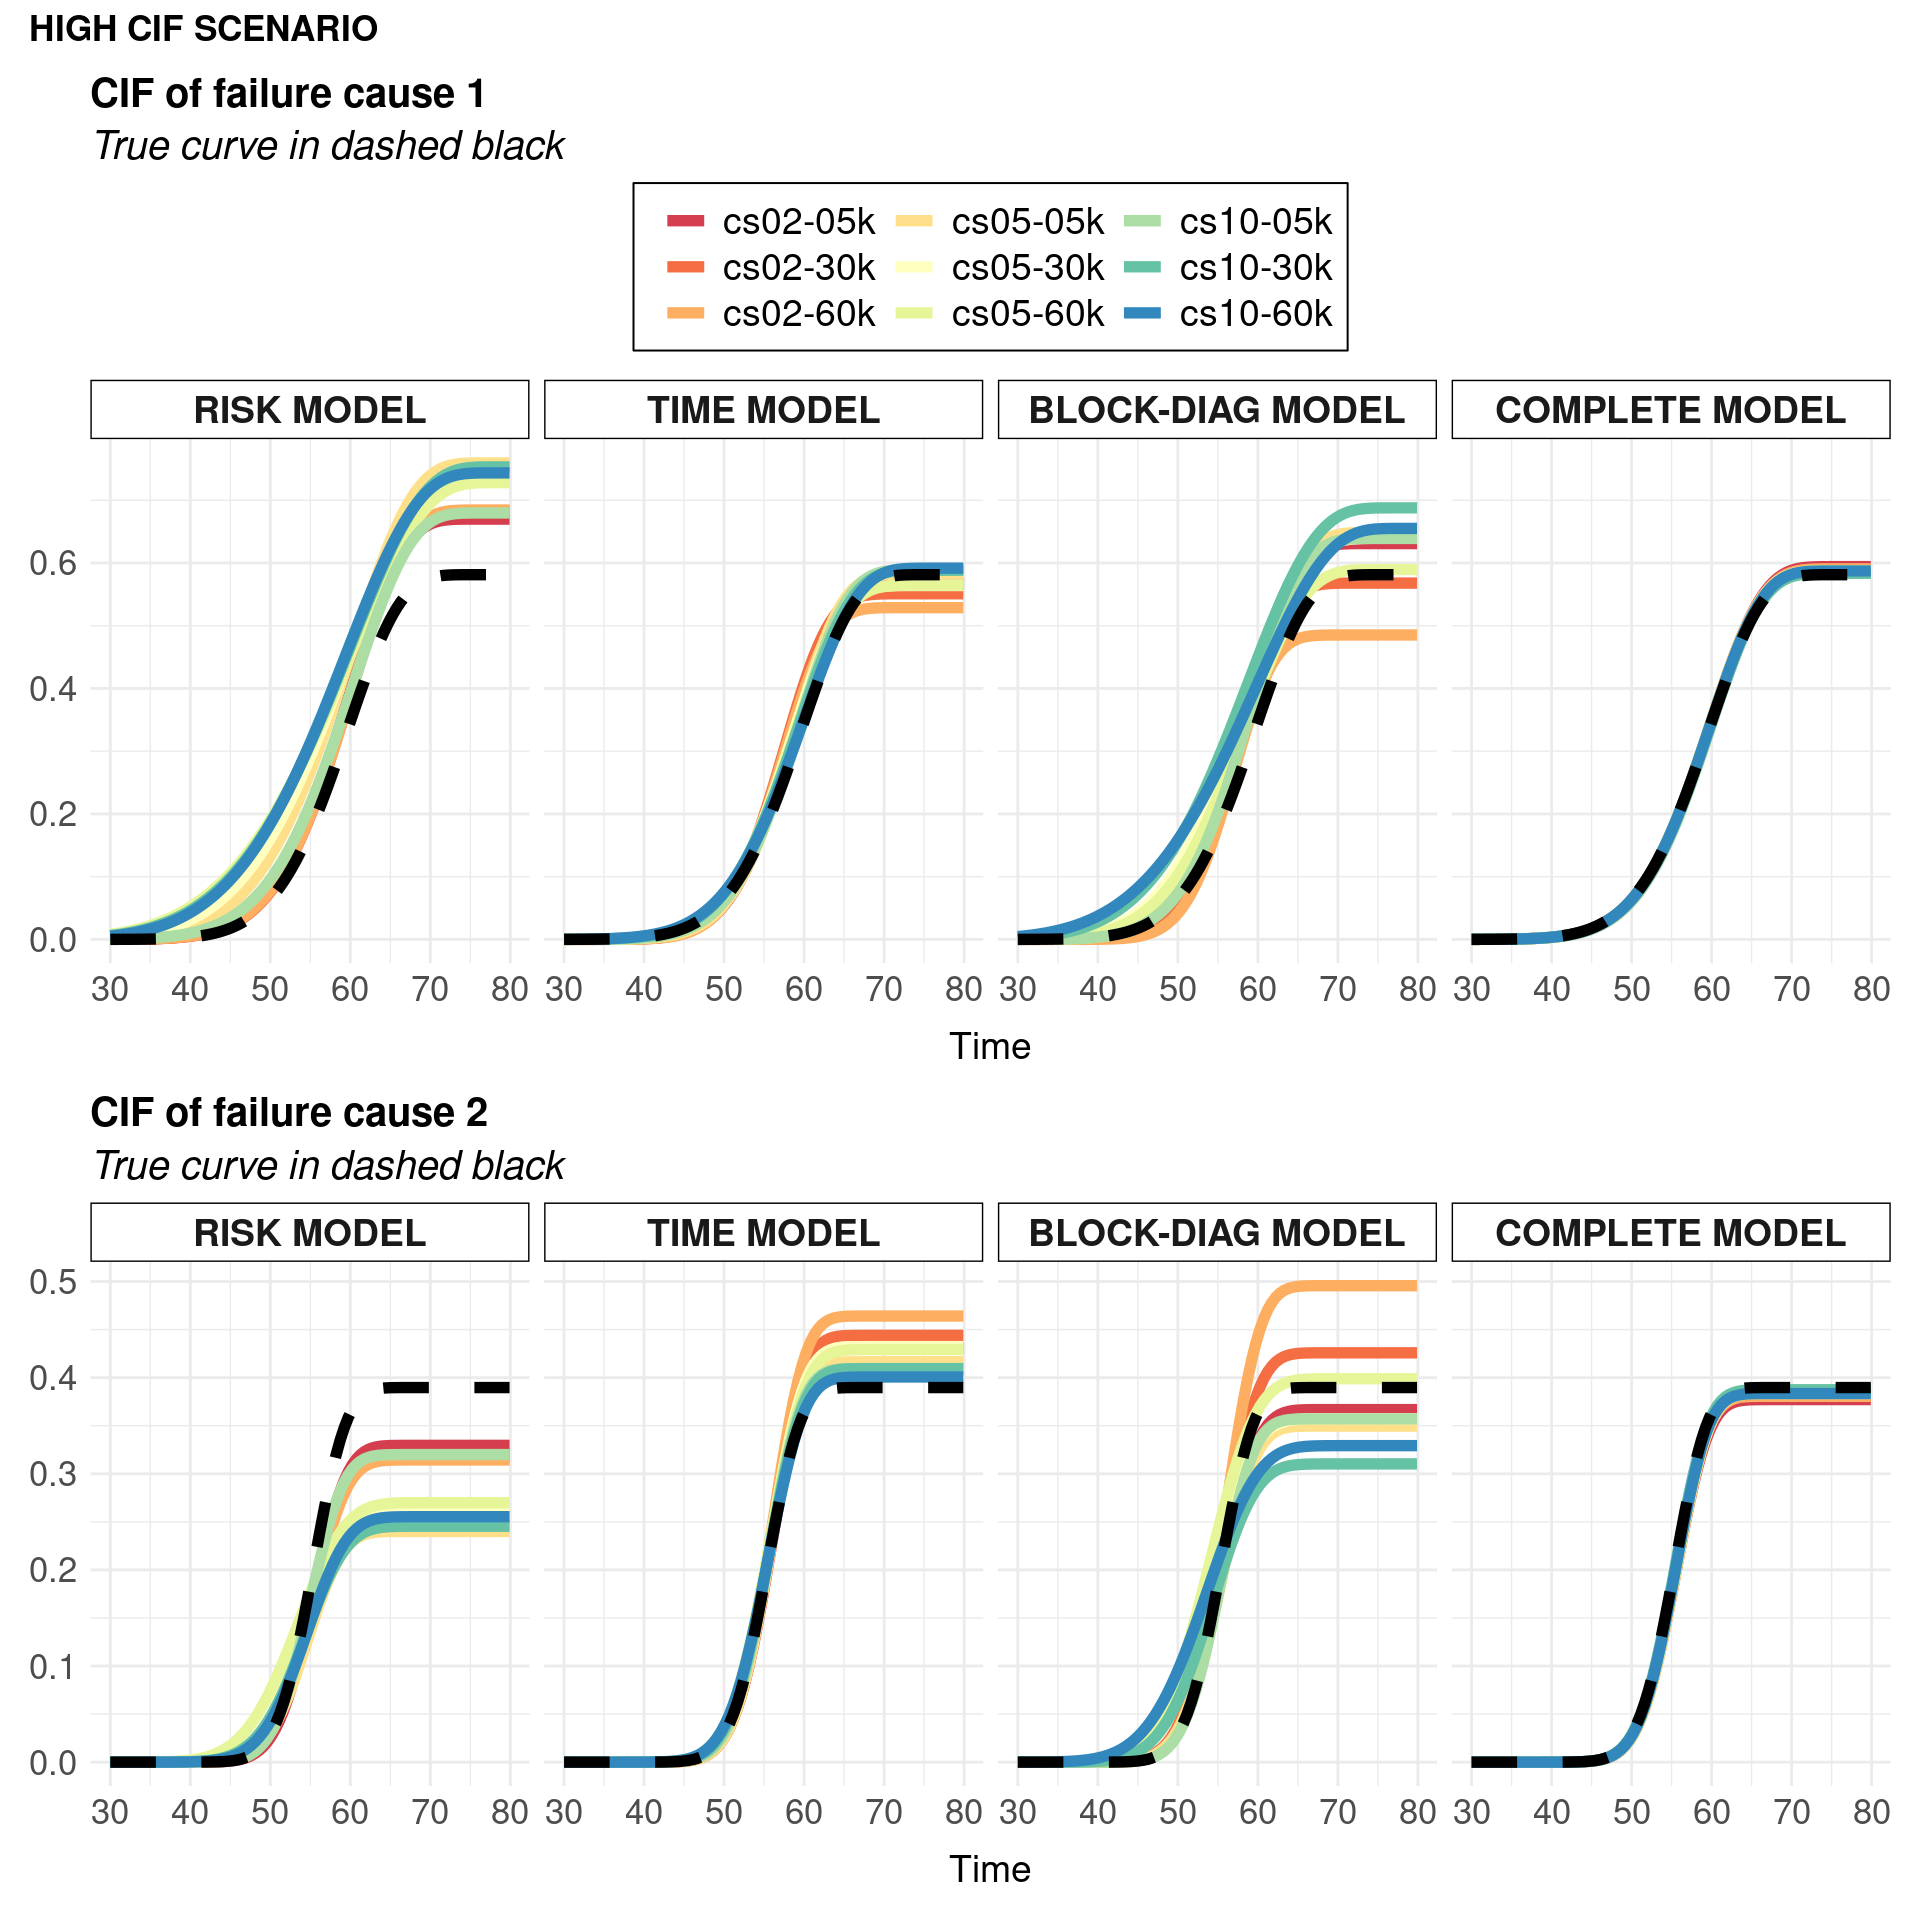
\includegraphics[width=\textwidth]{cifs-1.png}\\
 \begin{footnotesize}
  SOURCE: The author (2021).
 \end{footnotesize}
 \label{fig:cifshigh}
\end{figure}

\begin{figure}[H]
 \setlength{\abovecaptionskip}{.0001pt}
 \caption{LOW CUMULATIVE INCIDENCE FUNCTION (CIF) SCENARIO CURVES}
 \vspace{0.2cm}\centering
 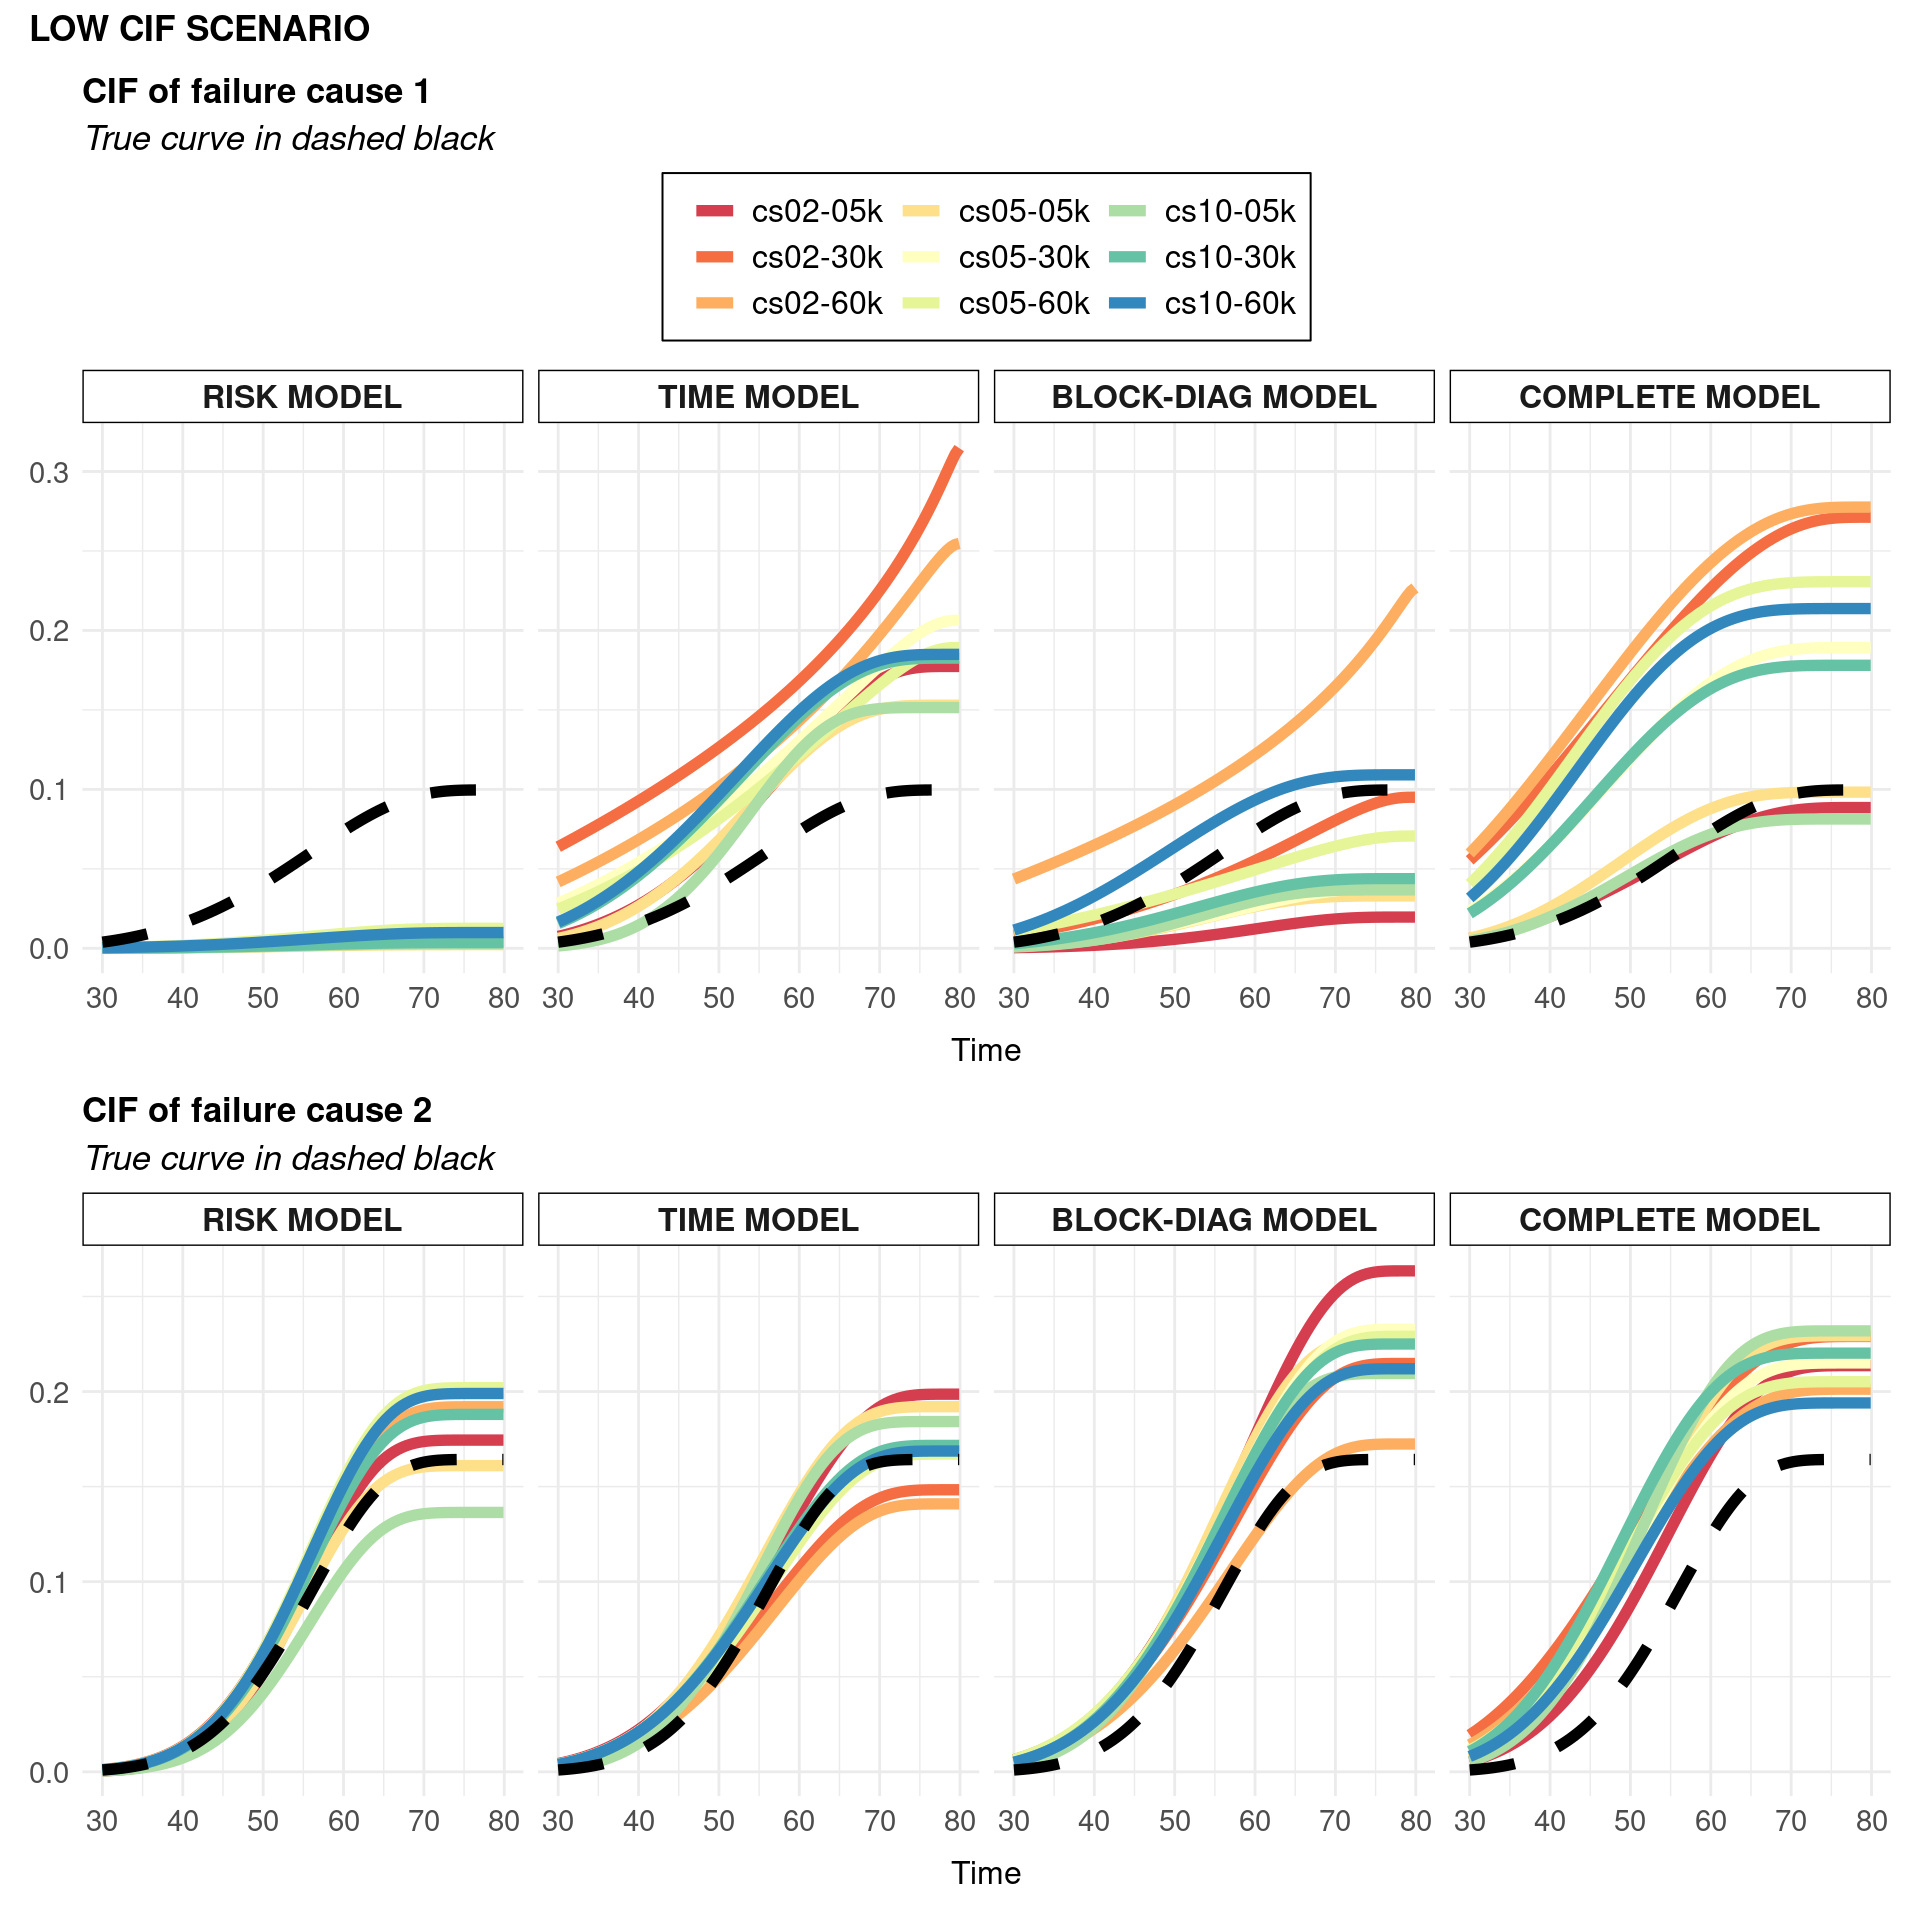
\includegraphics[width=\textwidth]{cifs-2.png}\\
 \begin{footnotesize}
  SOURCE: The author (2021).
 \end{footnotesize}
 \label{fig:cifslow}
\end{figure}

Since for all the models we have a latent structure for the
within-cluster dependency, the inherent idea is that this also affect
the fixed-effect parameter estimates. By taking its average in each of
the seventy-two scenarios, we are able to construct the mean CIF curves.

In \autoref{fig:cifshigh} we have all the thirty-six curves obtained in
the high CIF scenarios. It is clear that with the complete model we get
a perfect fit in all nine scenarios. The risk and time models estimate
well the curve shape parameters but they fail to learn the max
incidence. A compensation between curves is clear. In the risk model,
there is a super estimation of \(\beta_{1}\) in all scenarios. For
failure cause 2, there is a sub estimation. With the time model, we
observe the opposite compensation but on a smaller scale.

With the time model, we get much better curves than with the risk
model. The block-diag model results are a middle term between them. For
the time model, the scenario with cluster size 10 and 60 thousand data
points is a highlight. For the block-diag model, the highlight is the
scenario with cluster size 5 and 30 thousand data points.

In the low CIF scenarios in \autoref{fig:cifslow}, the estimation is
clearly more difficult. The overall fits are bad, being impossible to
select a scenario with overall good results. For one of the failure
causes, the estimation quality is not so bad. The problem is when we
look to the other. An interesting scenario is the one with cluster size
2 and 60 thousand data points. In this scenario we see the worst fits
for failure cause 1, with a negative highlight in the block-diag
configuration. However, with this same model, for failure cause 2, it is
the only scenario, by far, were we learn the true curve. An interesting
compensation phenomena. The best joint fit is still with the complete
model.

Now we look at how the latent-effect parameter estimates distribute
themselves. Given the huge number of scenarios and the fact that is
harder to estimate covariance parameters, we chose to plot the
parameters just in the scenarios with better performances. By the
metrics of small bias and CIF shape learning, the scenarios with better
results are the ones with high CIF and bigger sample sizes. We have the
densities for the variance parameters, in each of these scenarios,
presented in \autoref{fig:histologs2}. In \autoref{fig:historhoz} we
have the same for the correlation parameters.

An interesting result is the clear difference between risk and time
models' covariance parameters. With the risk model, we have an evident
super estimation and bigger variances. With the time model we get much
better results, but still with high variances. The block-diag model
generally performs better than the risk model and worst than the time
model, showing again to be a compromise between them. Besides the bias
itself, we should also pay attention to the values. We model the
variances in the log-scale, so a value 5, in reality, implies a variance
of \(\exp(4) = 148\). Terrible. This kind of problem do not sound to
appear with the complete model.

All correlations are quite well estimated, in all three scenarios, with
the complete model. Not only the correlations but the variances
also. The lack of any considerable difference between the covariance
densities, indicates no quality divergences in the results for different
cluster sizes. The densities in \autoref{fig:histologs2} and
\autoref{fig:historhoz} are the final corroboration indicating the good
estimability of the complete model. Between the four tested models, the
complete model was the one with the smallest biases, better CIF shape
learning, and precisest covariance parameter estimates.

In \autoref{fig:cor2plot} we have a heat-map of the correlations between
parameter estimates for the complete model in the scenario with clusters
of size 10, high CIF, and 60 thousand data points.

\begin{figure}[!htpb]
 \setlength{\abovecaptionskip}{.0001pt}
 \caption{VARIANCE PARAMETERS DENSITIES IN THE SCENARIOS OF HIGH CIF AND
          60 THOUSAND DATA POINTS}
 \vspace{0.2cm}\centering
 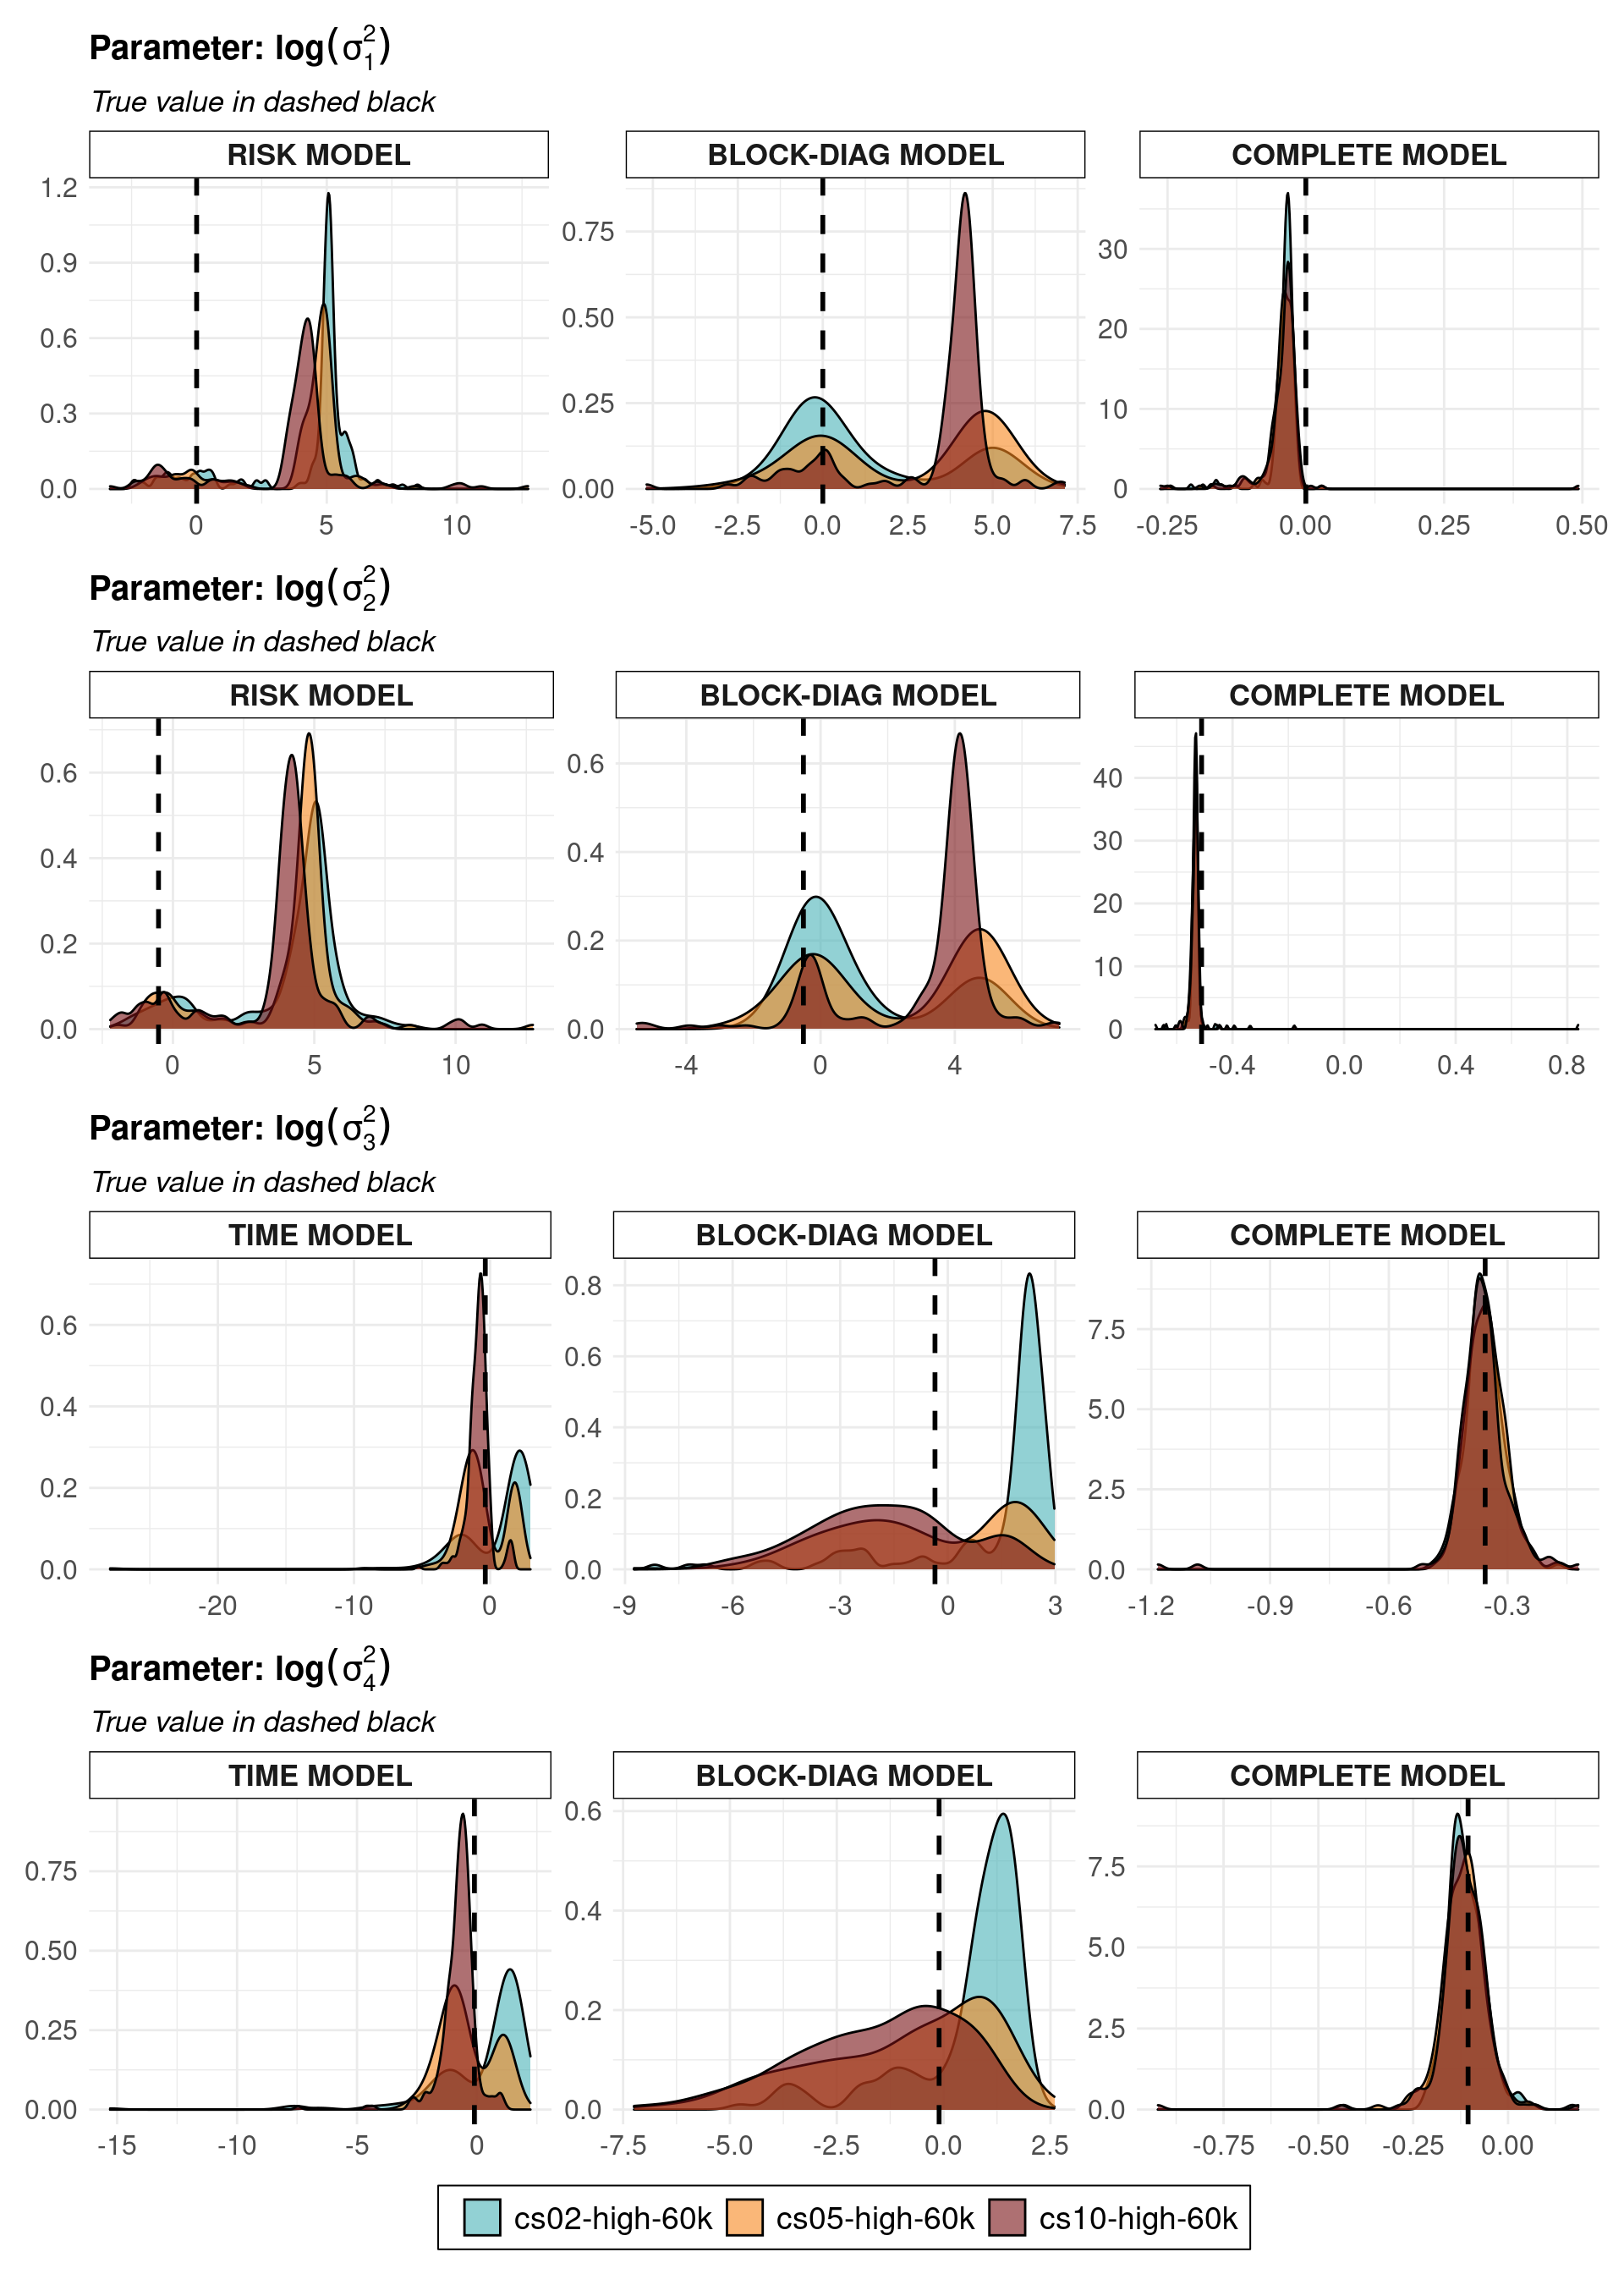
\includegraphics[width=\textwidth]{histologs2-1.png}\\
 \begin{footnotesize}
  SOURCE: The author (2021).
 \end{footnotesize}
 \label{fig:histologs2}
\end{figure}

\begin{figure}[H]
 \setlength{\abovecaptionskip}{.0001pt}
 \caption{CORRELATION PARAMETERS DENSITIES IN THE SCENARIOS OF HIGH CIF
          AND 60 THOUSAND DATA POINTS}
 \vspace{0.2cm}\centering
 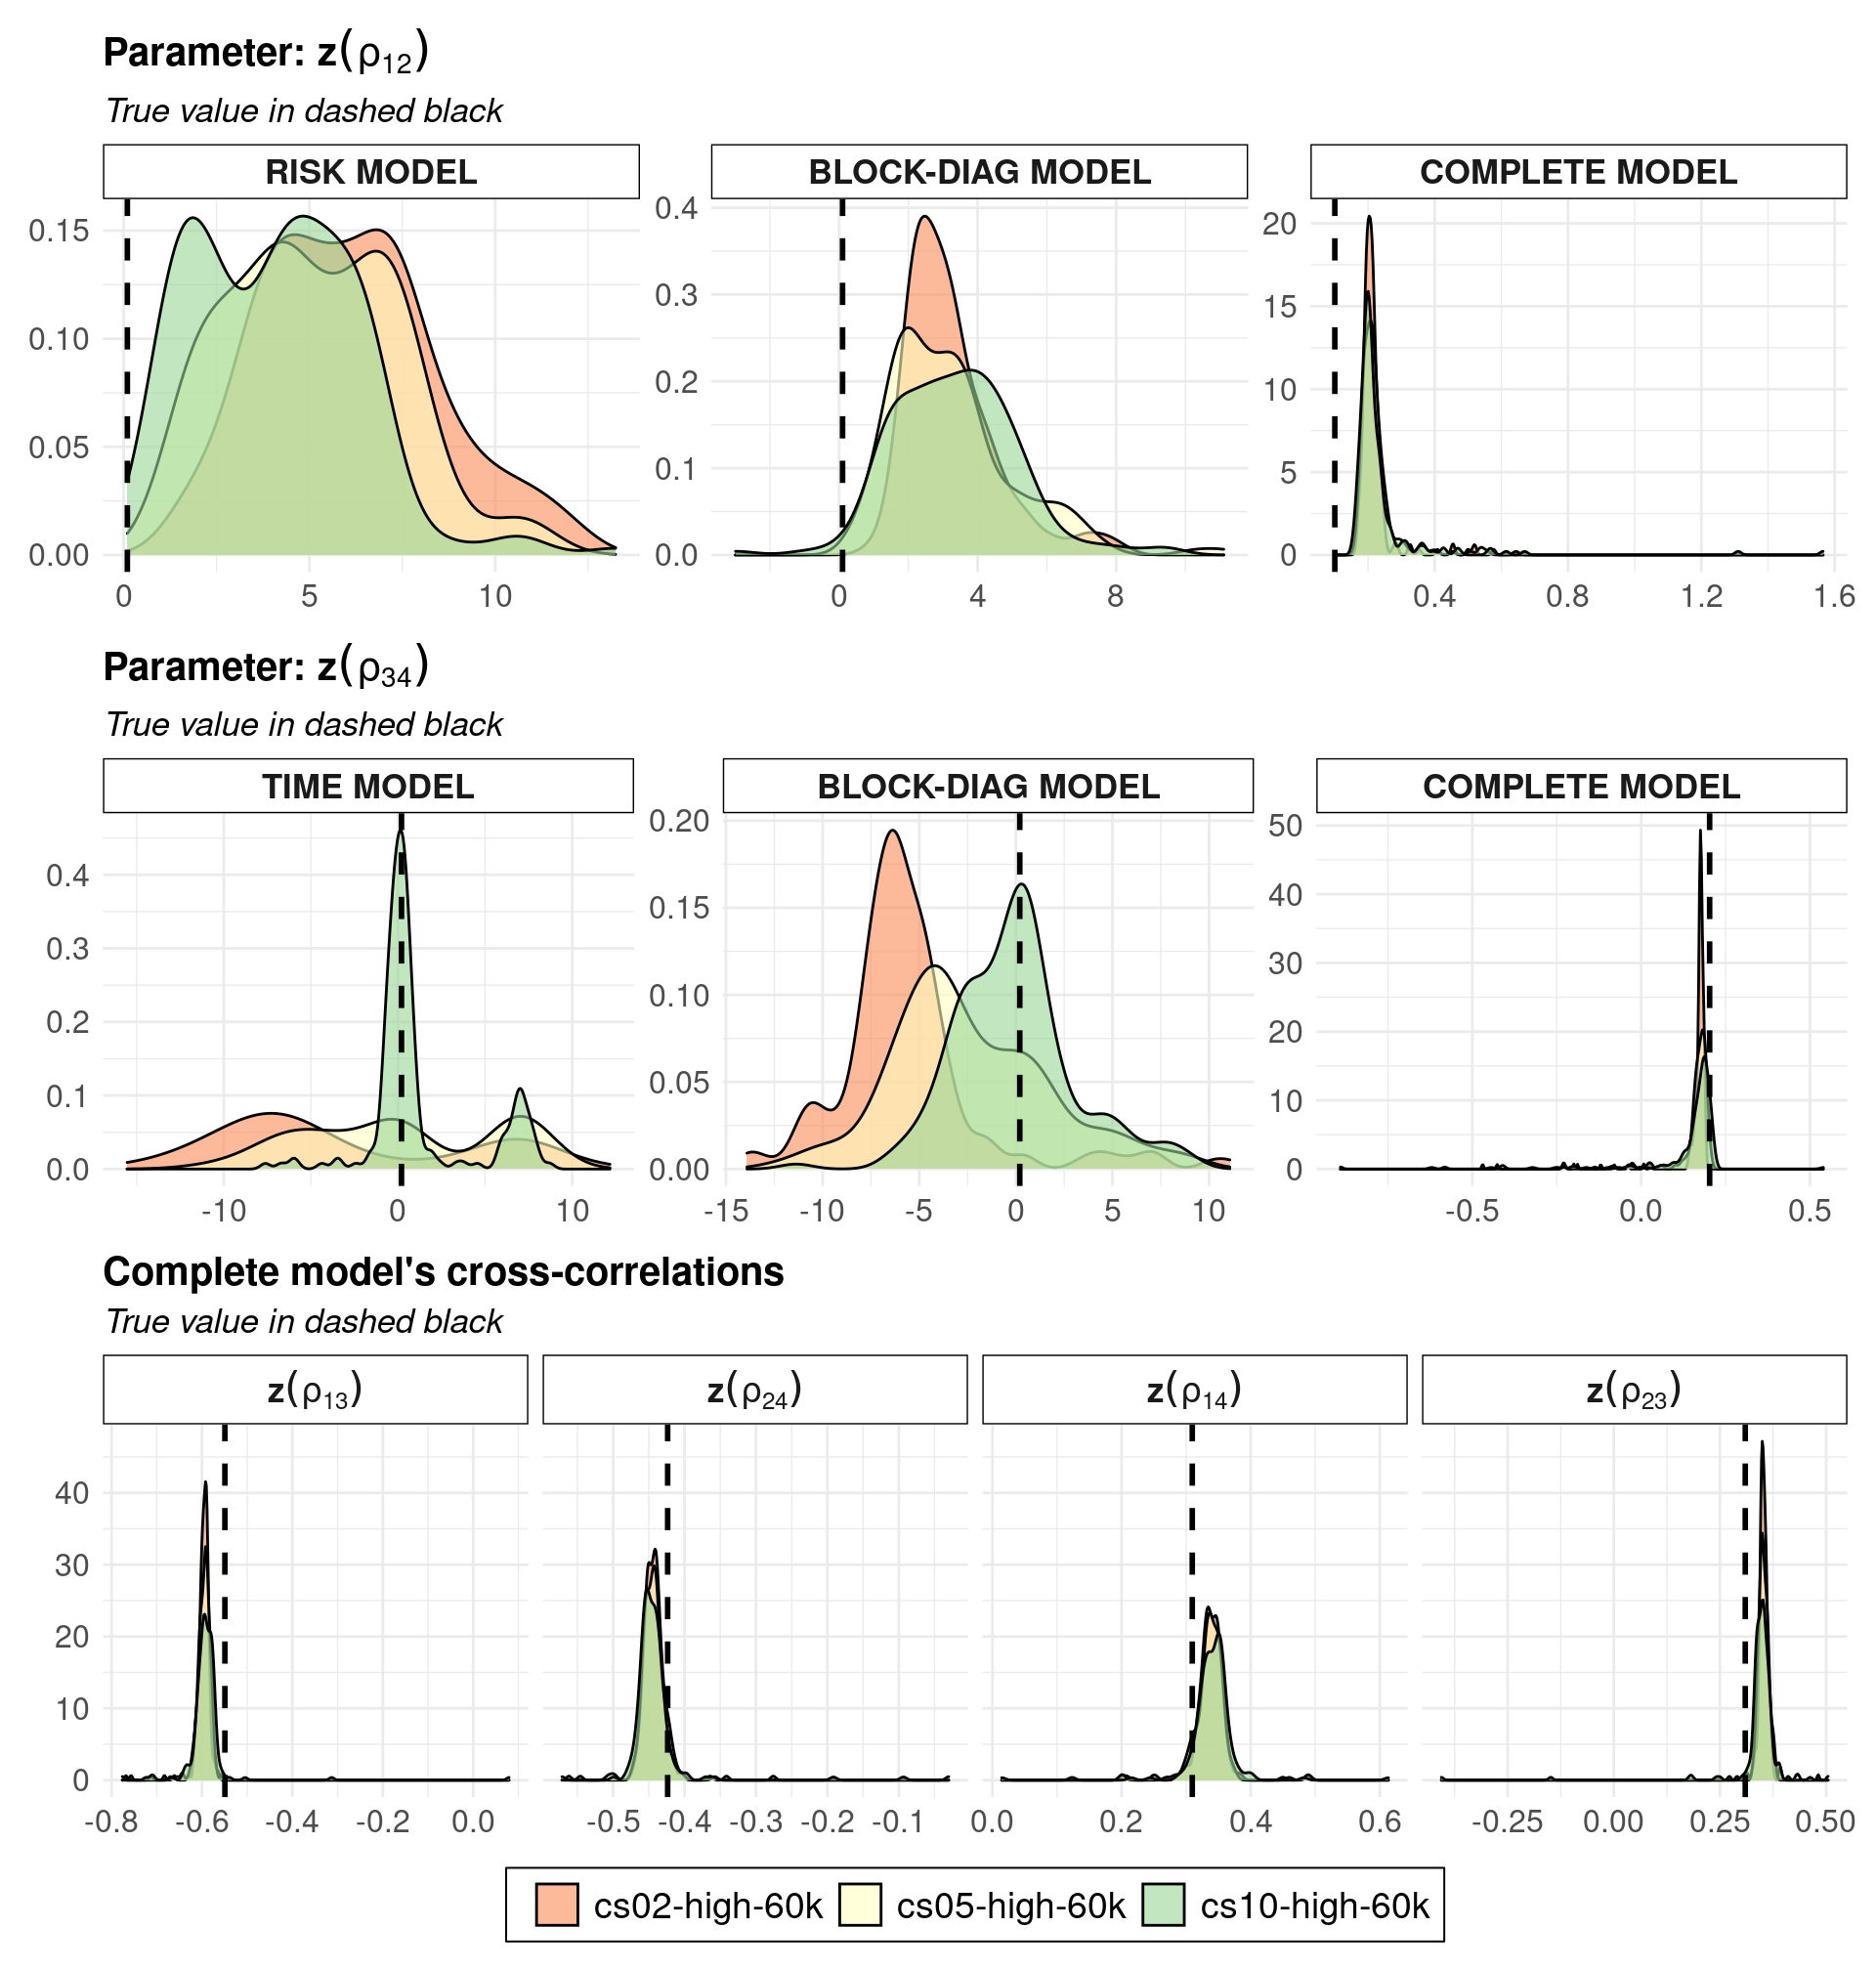
\includegraphics[width=\textwidth]{historhoz-1.png}\\
 \begin{footnotesize}
  SOURCE: The author (2021).
 \end{footnotesize}
 \label{fig:historhoz}
\end{figure}

We have a little bit of everything in \autoref{fig:cor2plot}. Some
correlations are very close to zero, but we also have strong positive
and negative correlations. We can mention some curiosities, but nothing
pathological appears to happen, at least nothing clear.

All fixed-effect parameters are positive correlated, with an emphasis on
the correlation between \(\beta_{1}\) and \(\beta_{2}\), and the one of
the \(\bm{\beta}\)s with the \(\bm{w}\)s. Another interesting
observation is the negative correlation between the \(\bm{\beta}\)s and
the risk log-variances, and also the positive correlation between the
\(\bm{\beta}\)s and the trajectory time log-variances. The risk
log-variances are positively correlated. So do the time trajectory
ones. The correlations between the log-variances of different levels are
negative.

\begin{figure}[H]
 \setlength{\abovecaptionskip}{.0001pt}
 \caption{COMPLETE MODEL'S PARAMETERS CORRELATION HEAT-MAP IN THE
          SCENARIO OF CLUSTER SIZE 10, HIGH CIF, AND SIXTY-THOUSAND DATA
          POINTS}
 \centering
 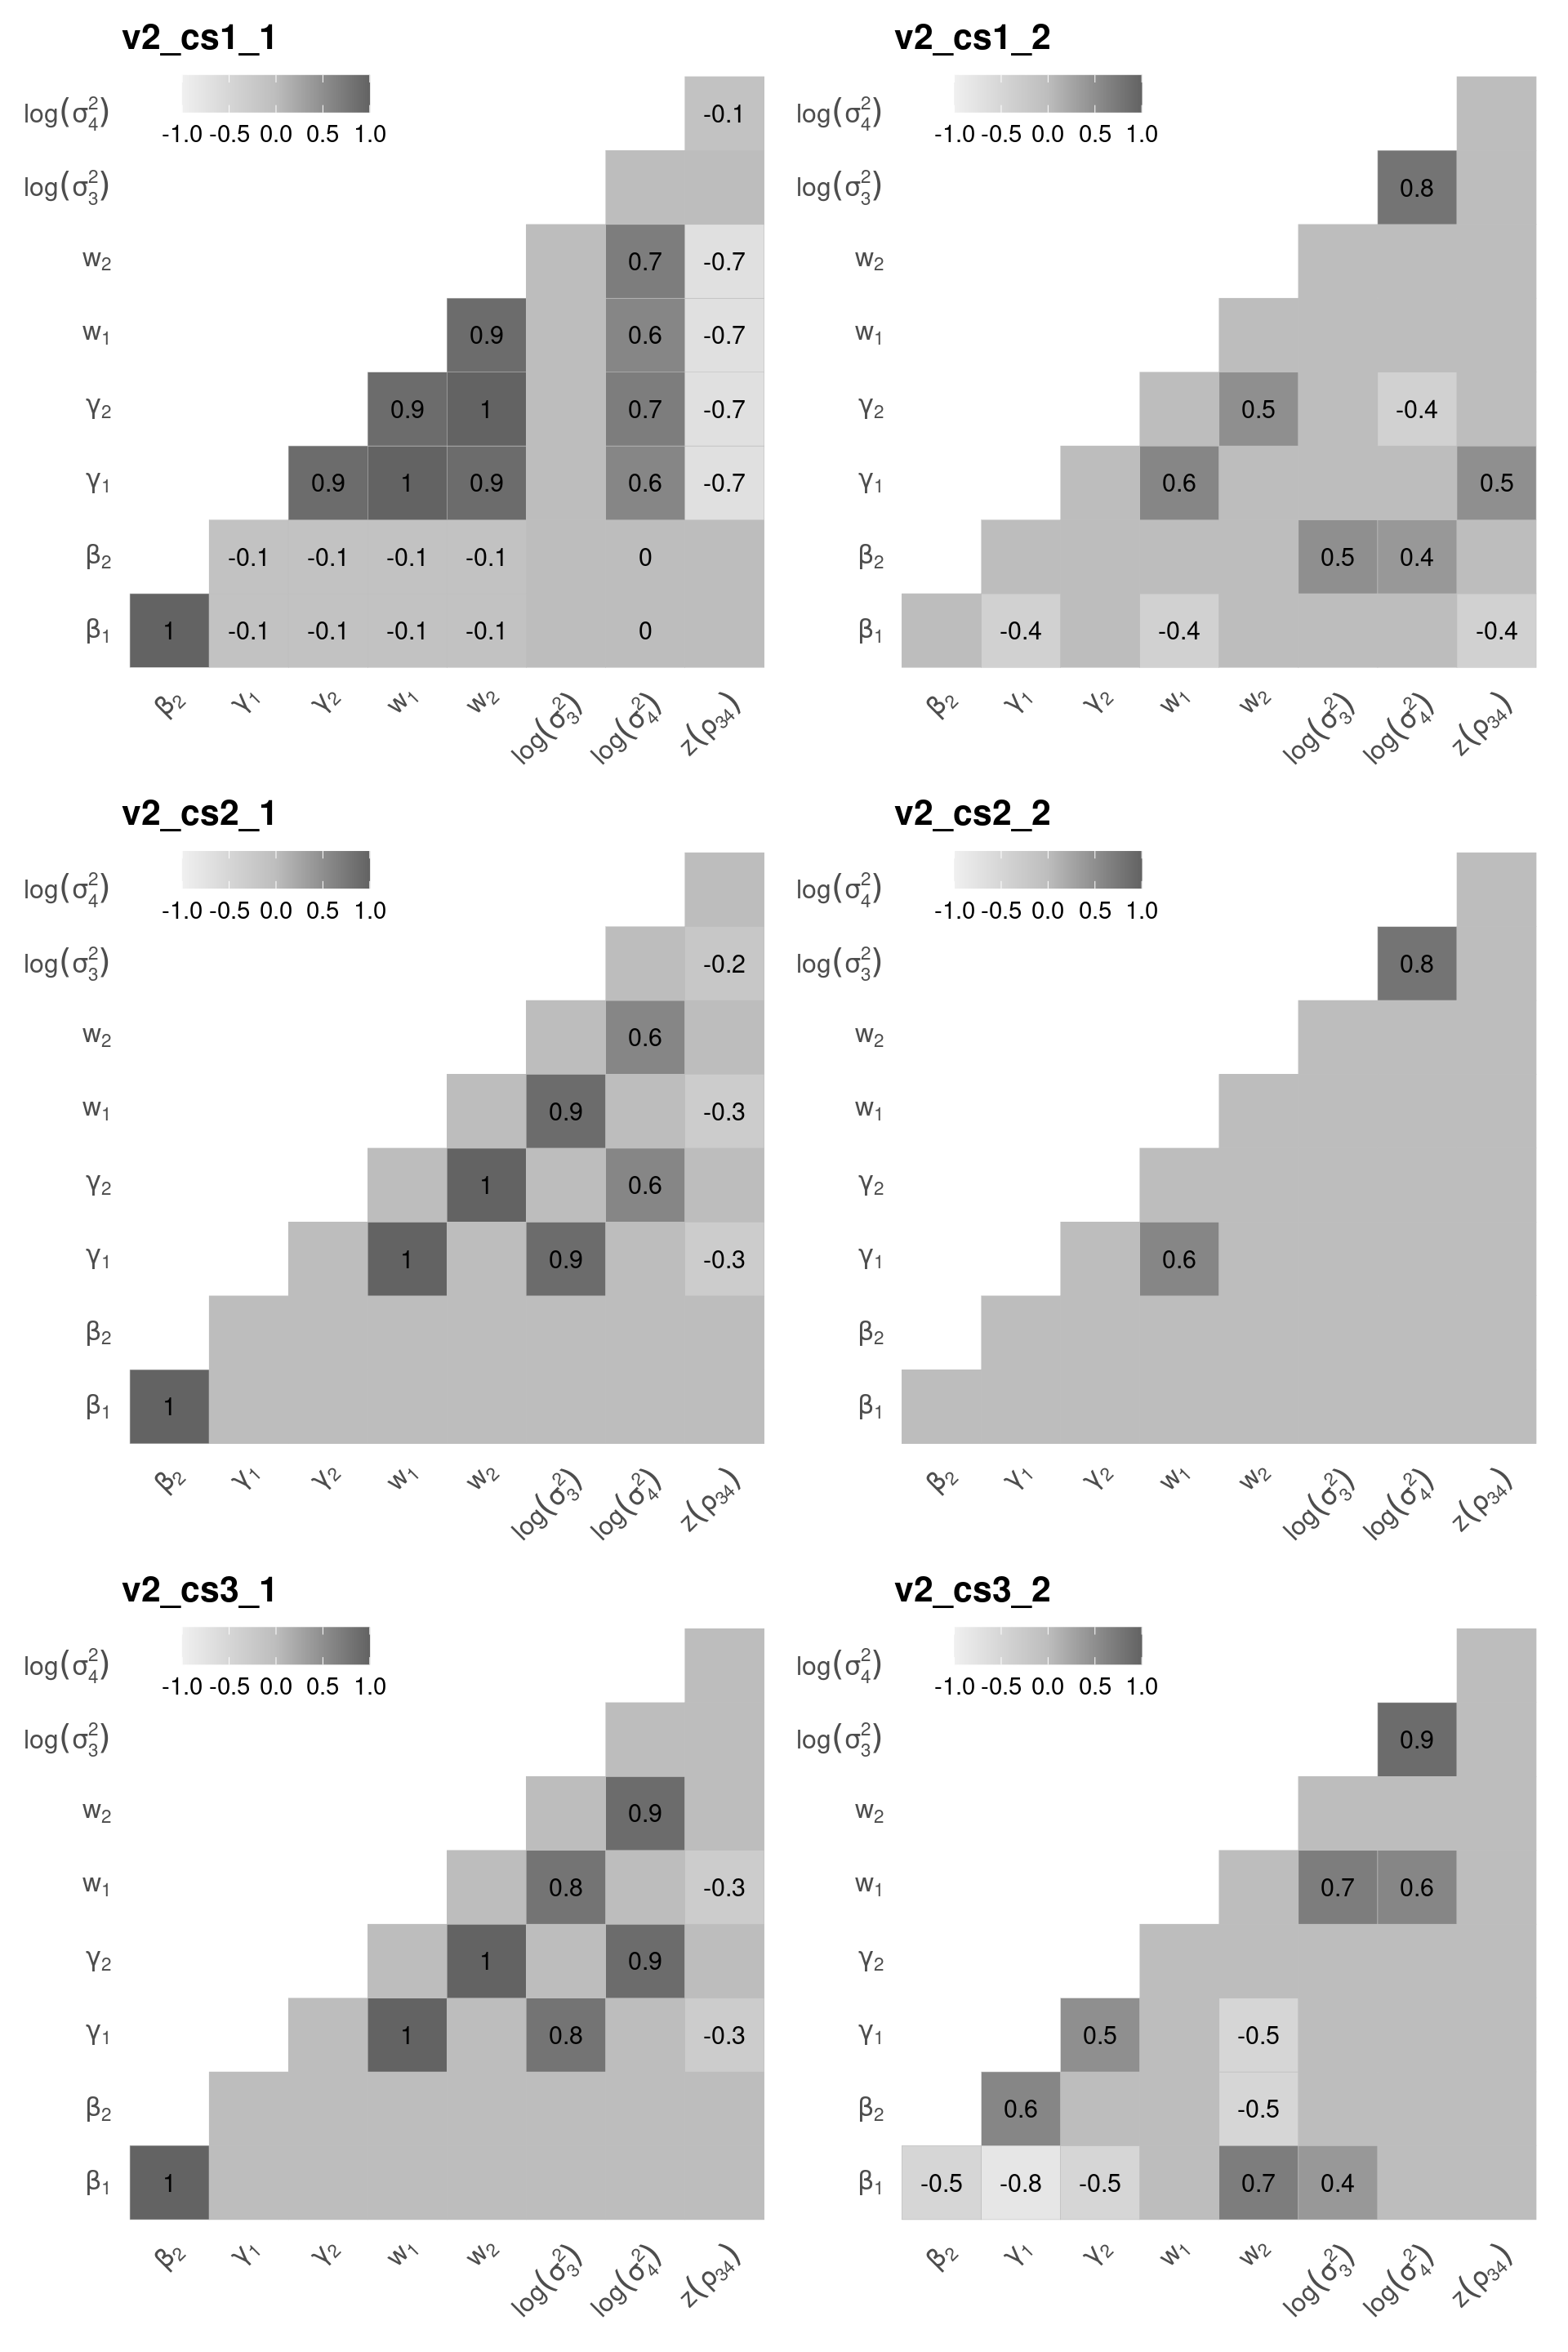
\includegraphics[width=\textwidth]{cor2plot-1.png}\\
 \vspace{-0.2cm}
 \begin{footnotesize}
  SOURCE: The author (2021).
 \end{footnotesize}
 \label{fig:cor2plot}
\end{figure}

% END ==================================================================
